\chapter{Zeichnungen}\label{sec:zeichnungen}
\newpage
\setlength{\voffset}{0cm}
\setlength{\hoffset}{0cm}
%
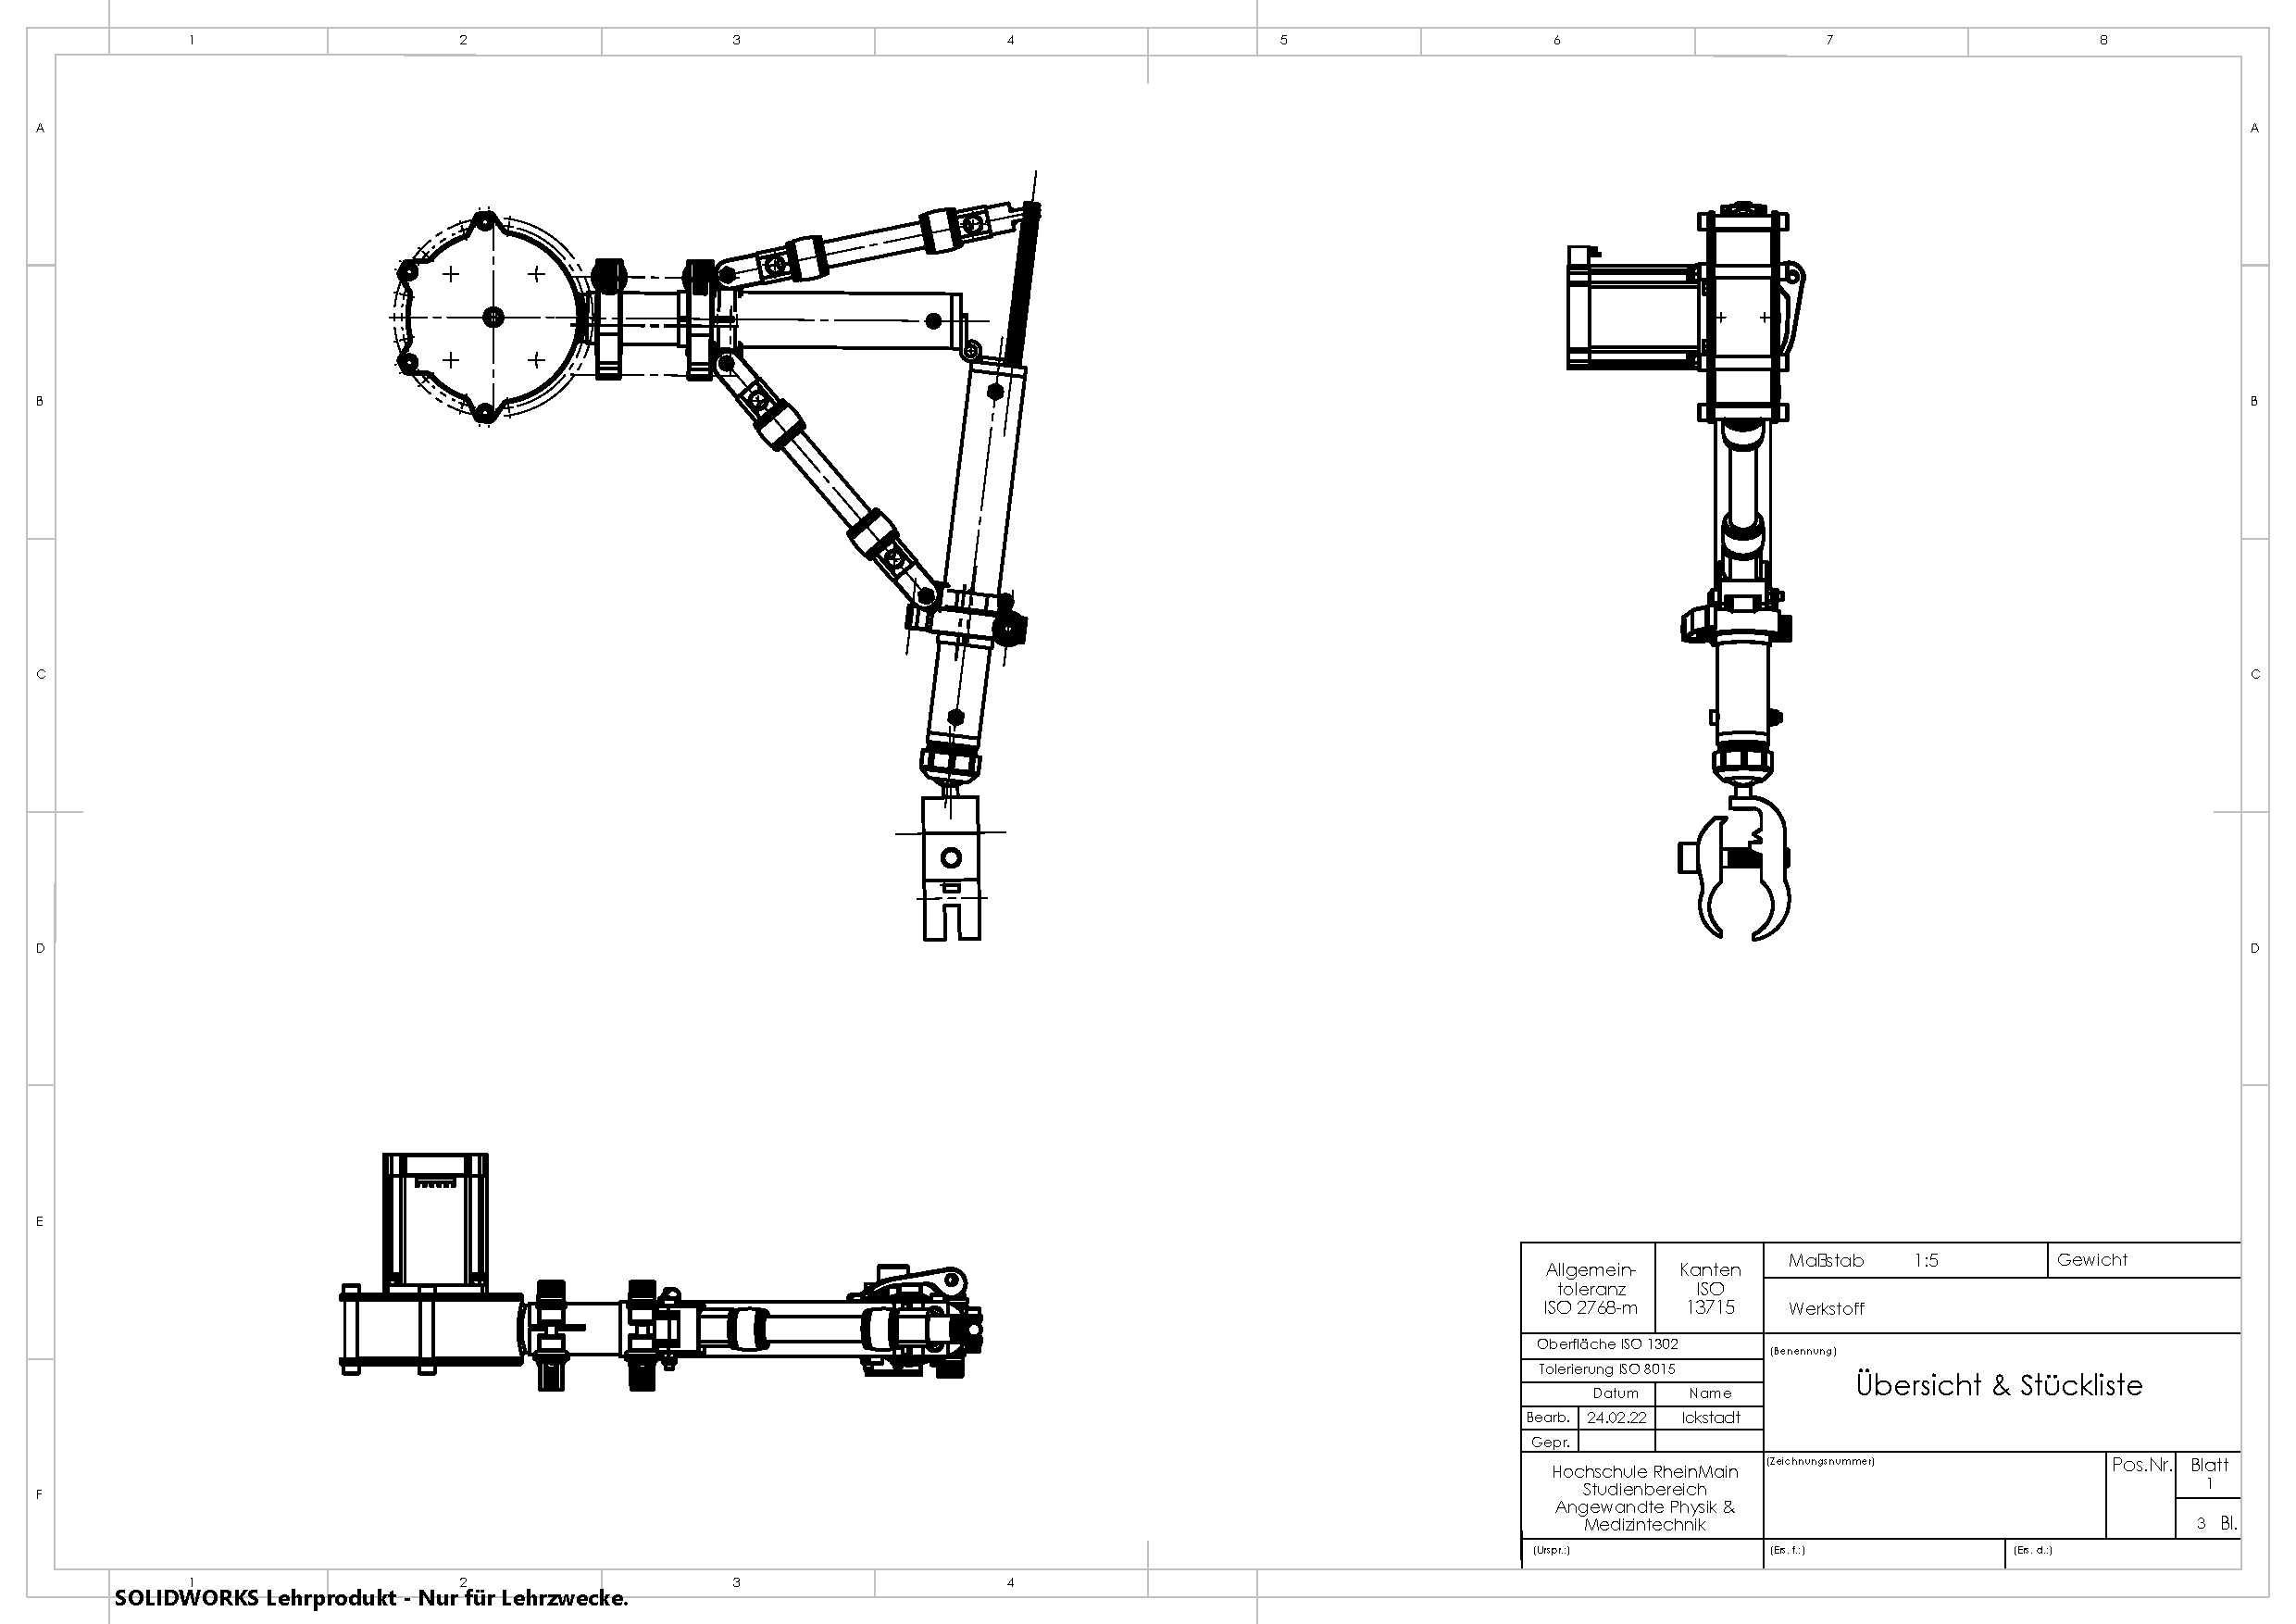
\includepdf[pages=1, angle=90, pagecommand={\thispagestyle{plain}}, addtolist={1, figure, Übersicht und Stückliste, drw:Uebersicht und Stueckliste}, addtotoc={1, section, 1, Bauteilzeichnungen, sec:bauteilzeichnungen}]{Abb/CAD/Drawings/Uebersicht-und-Stueckliste.pdf}
\includepdf[pages=2, angle=90, pagecommand={\thispagestyle{plain}}]{Abb/CAD/Drawings/Uebersicht-und-Stueckliste.pdf}
%
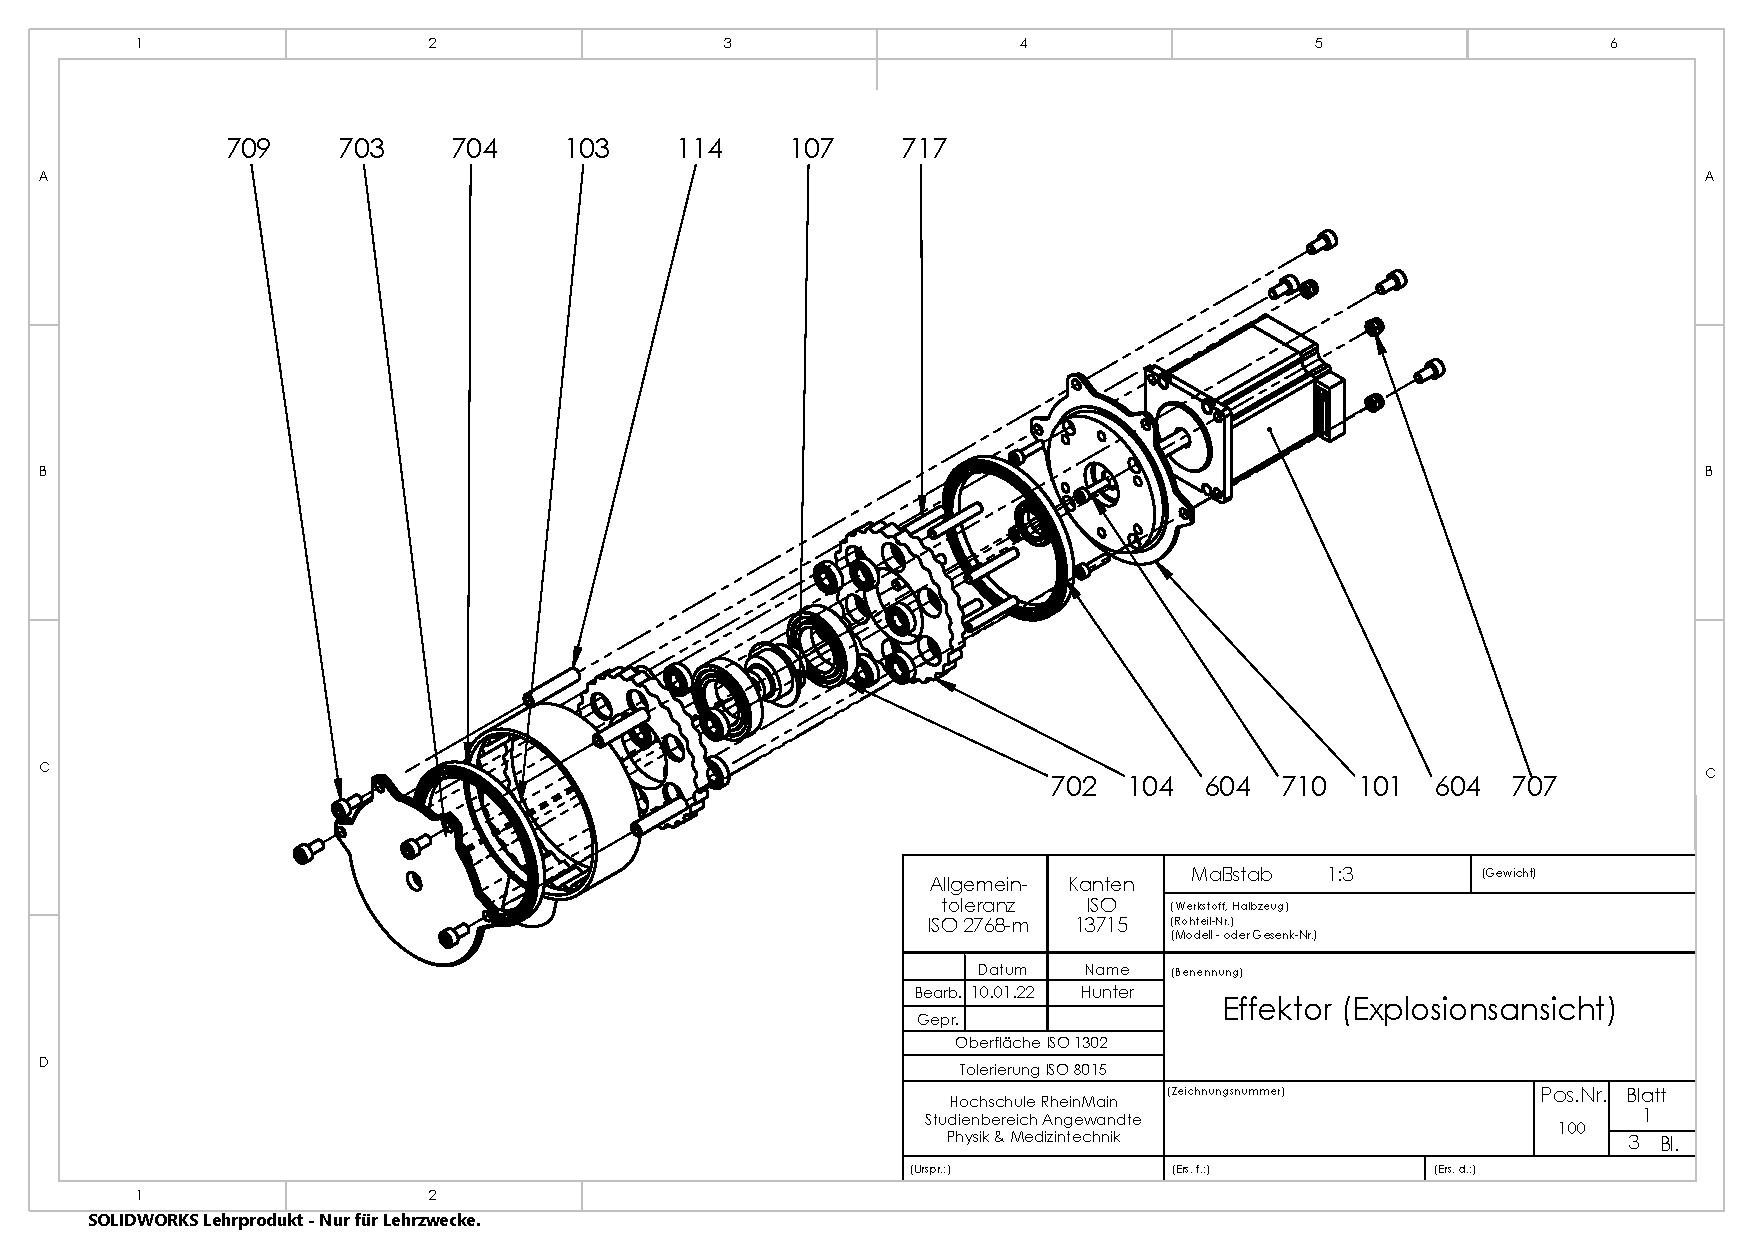
\includepdf[pages=1, angle=90, pagecommand={\thispagestyle{plain}}, addtolist={1, figure, Effektor, drw:Effektor}]{Abb/CAD/Drawings/Schulter/Effektor-assembly-drawing.pdf}
\includepdf[pages=2-3, angle=0, pagecommand={\thispagestyle{plain}}]{Abb/CAD/Drawings/Schulter/Effektor-assembly-drawing.pdf}
%
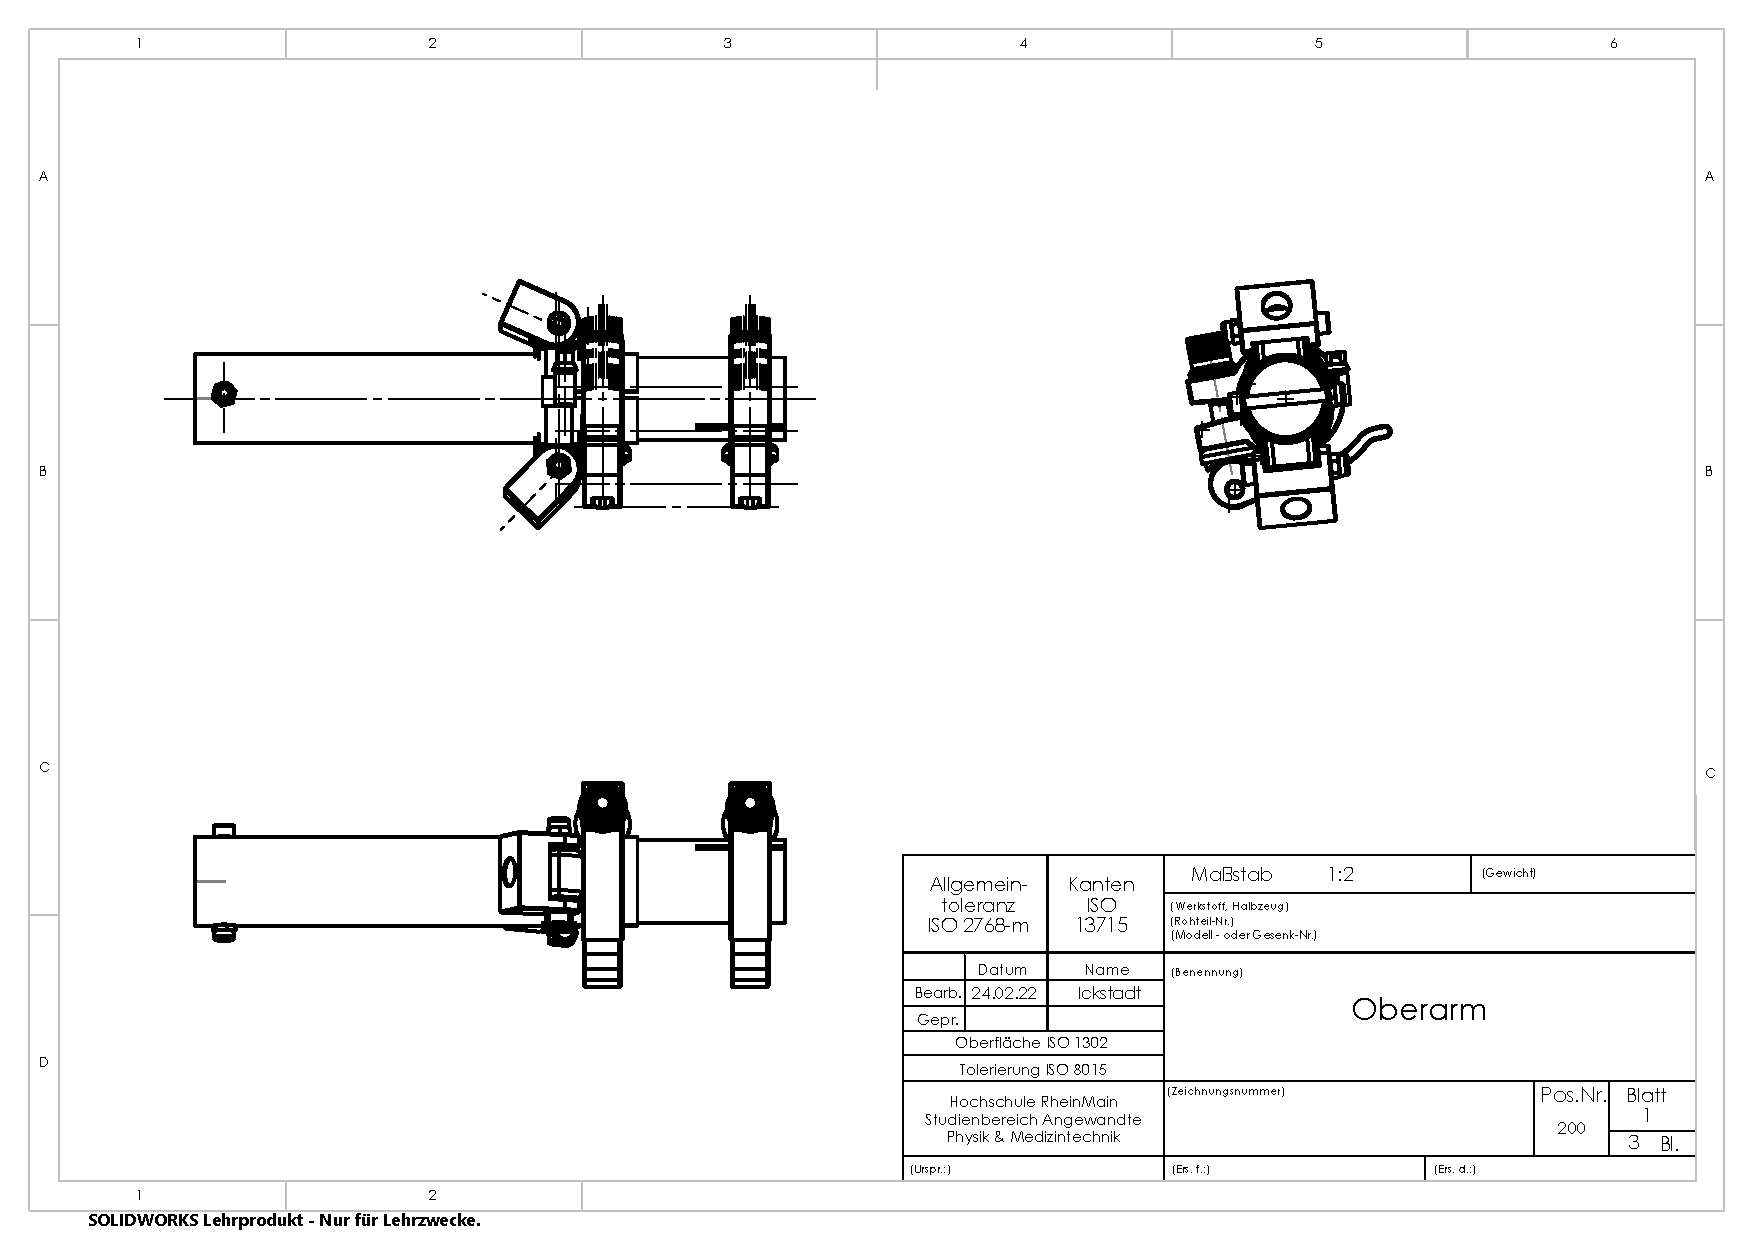
\includepdf[pages=1-2, angle=90, pagecommand={\thispagestyle{plain}}, addtolist={1, figure, Oberarm, drw:Oberarm}]{Abb/CAD/Drawings/Oberarm.pdf}
\includepdf[pages=3, angle=0, pagecommand={\thispagestyle{plain}}]{Abb/CAD/Drawings/Oberarm.pdf}
%
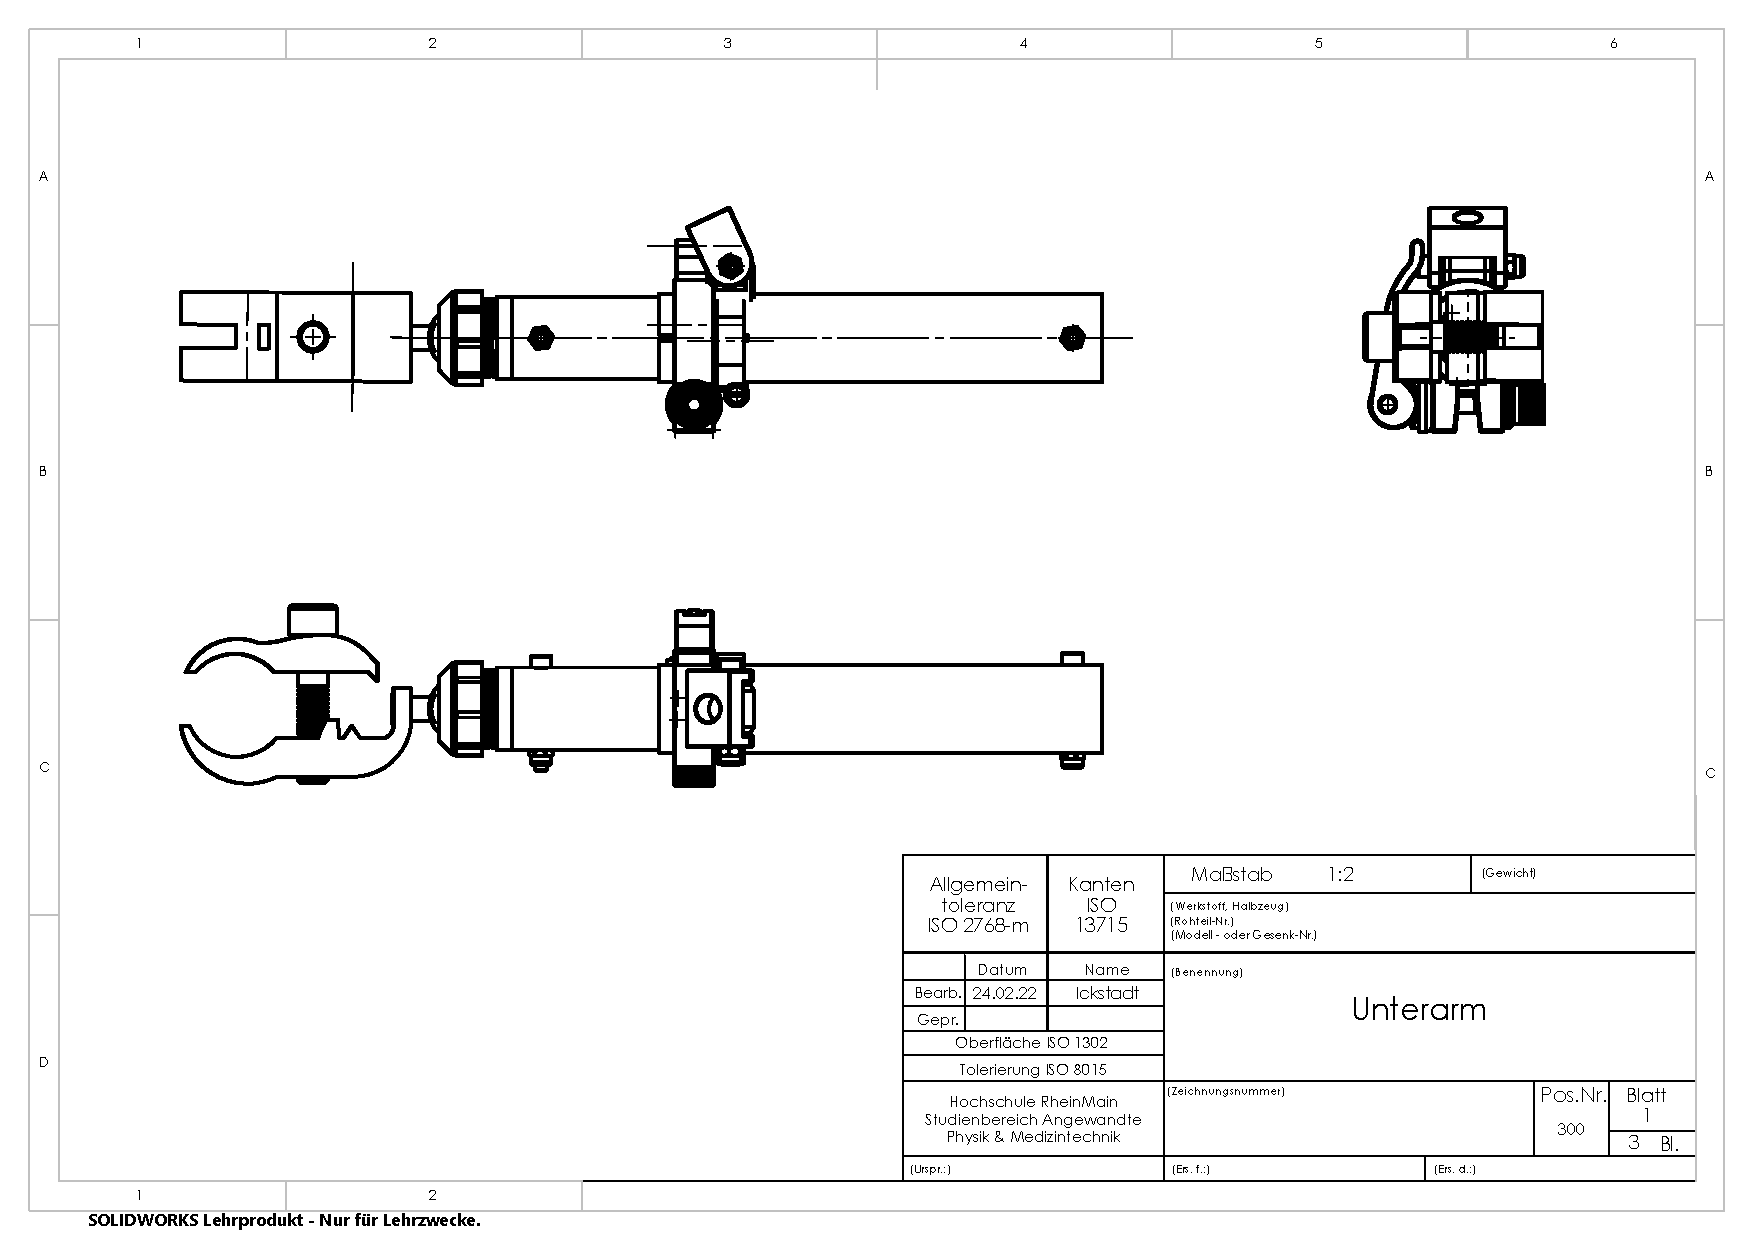
\includepdf[pages=1-2, angle=90, pagecommand={\thispagestyle{plain}}, addtolist={1, figure, Unterarm, drw:Unterarm}]{Abb/CAD/Drawings/Unterarm.pdf}
\includepdf[pages=3, angle=0, pagecommand={\thispagestyle{plain}}]{Abb/CAD/Drawings/Unterarm.pdf}
%
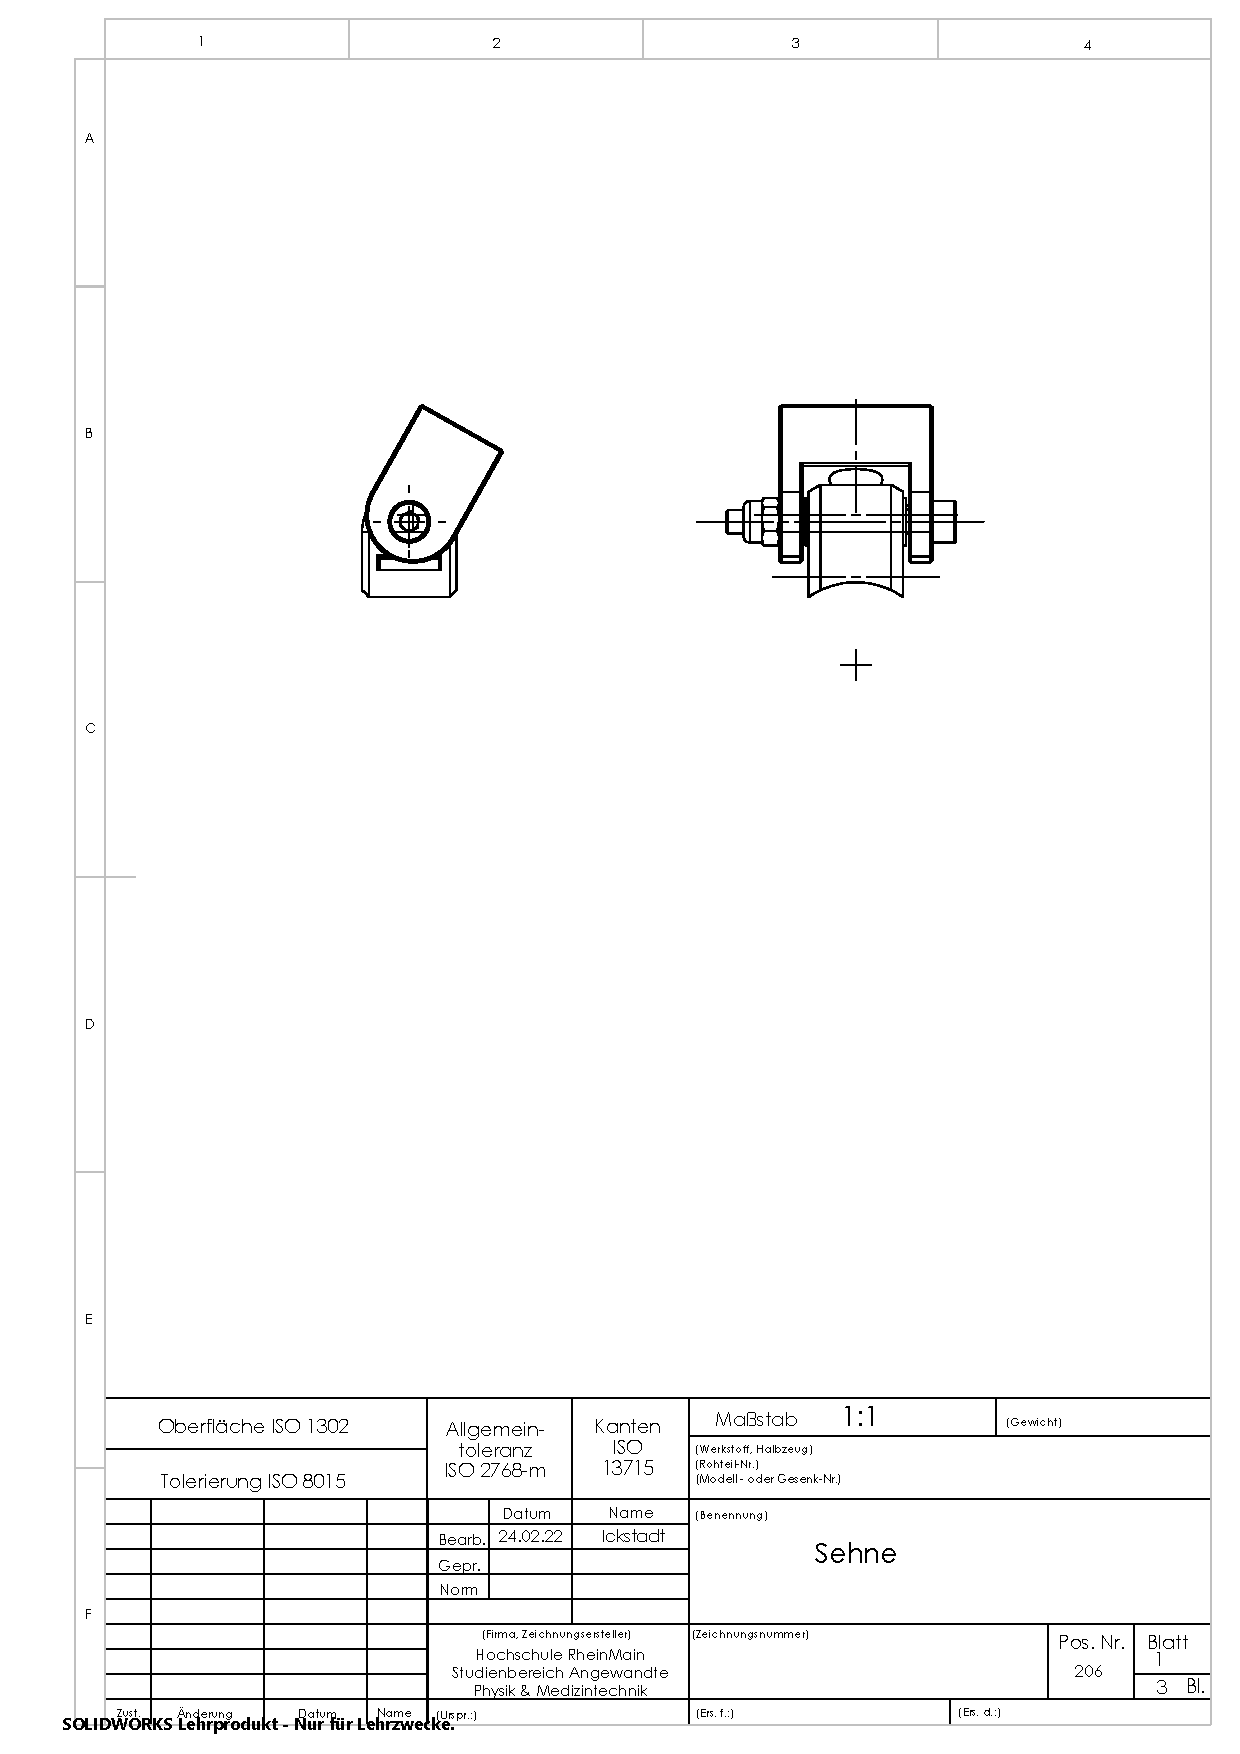
\includepdf[pages=-, angle=0, pagecommand={\thispagestyle{plain}}, addtolist={1, figure, Sehne, drw:Sehne}]{Abb/CAD/Drawings/Sehne.pdf}
%
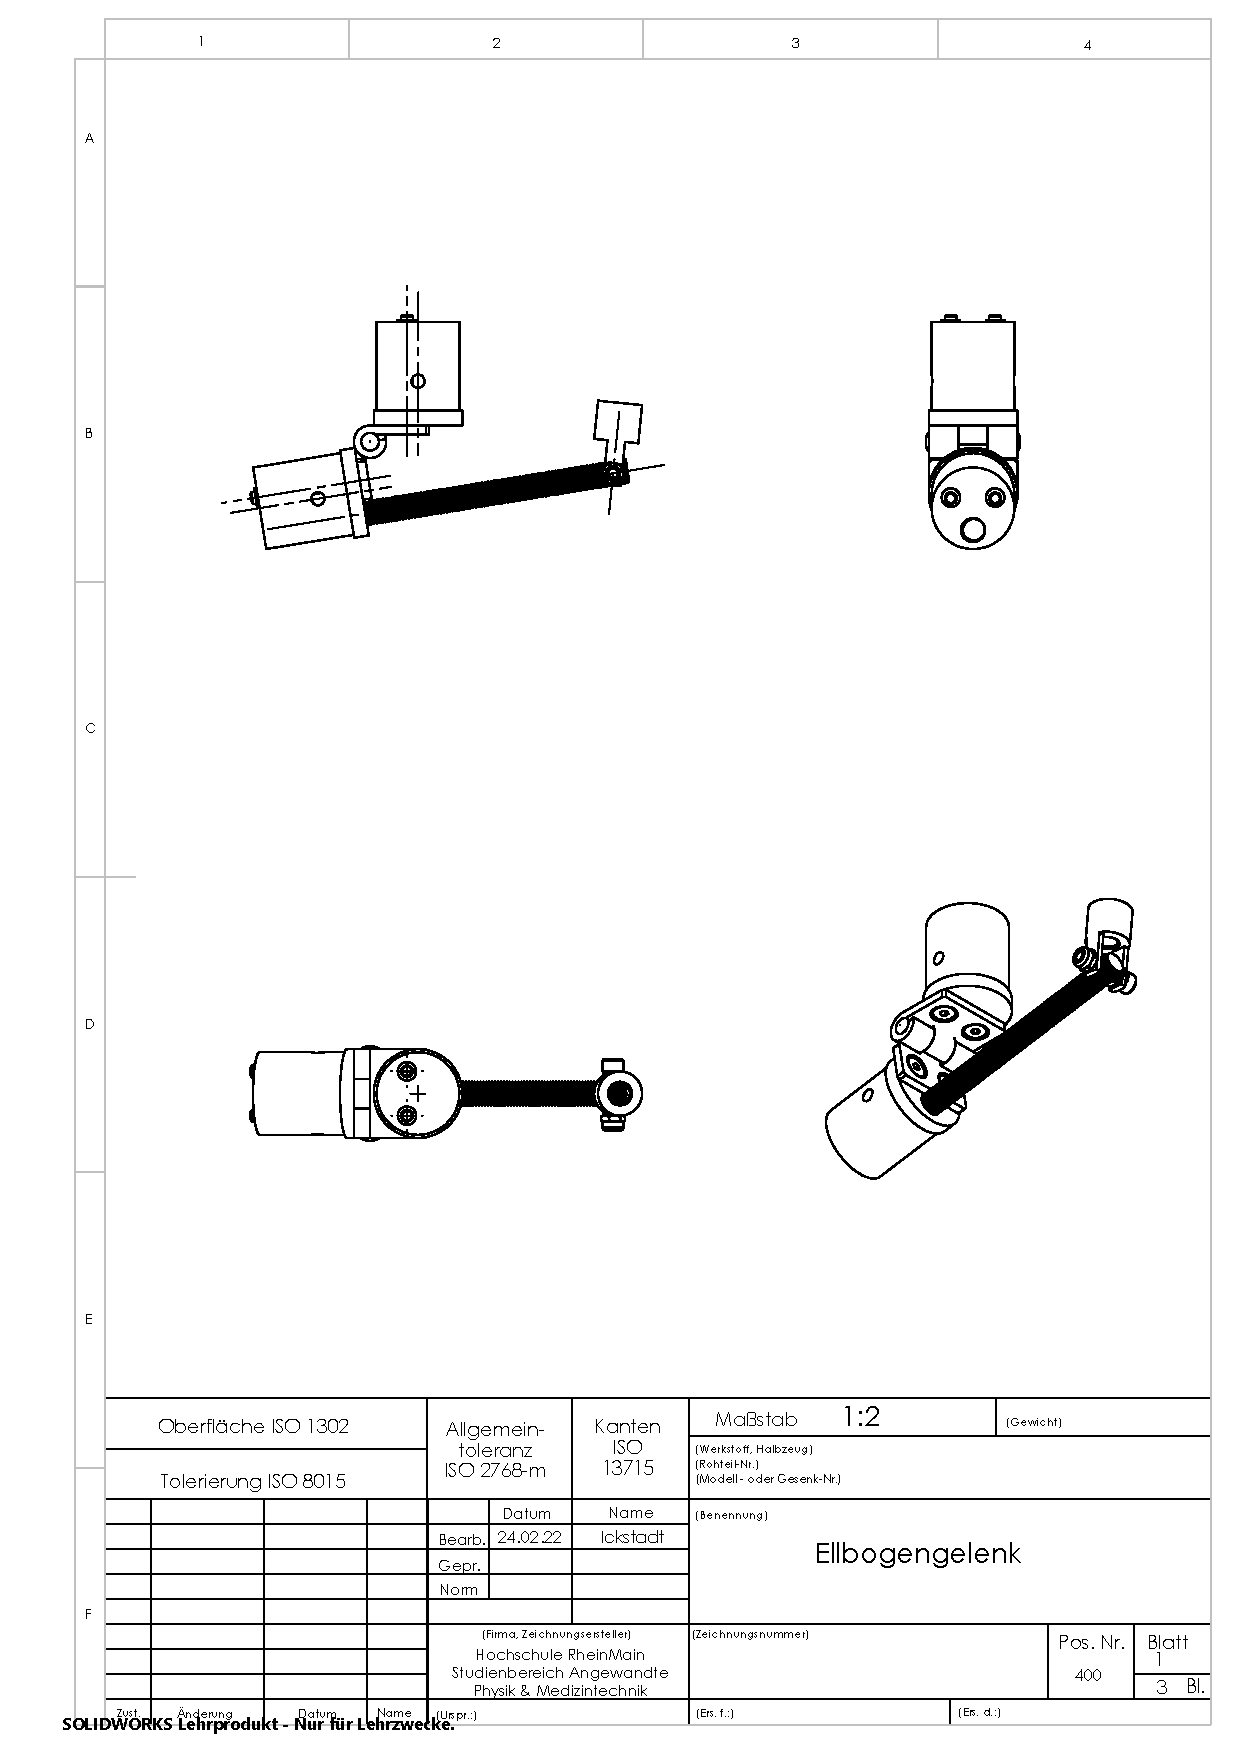
\includepdf[pages=-, angle=0, pagecommand={\thispagestyle{plain}}, addtolist={1, figure, Ellbogengelenk, drw:Ellbogengelenk}]{Abb/CAD/Drawings/Ellbogengelenk.pdf}
%
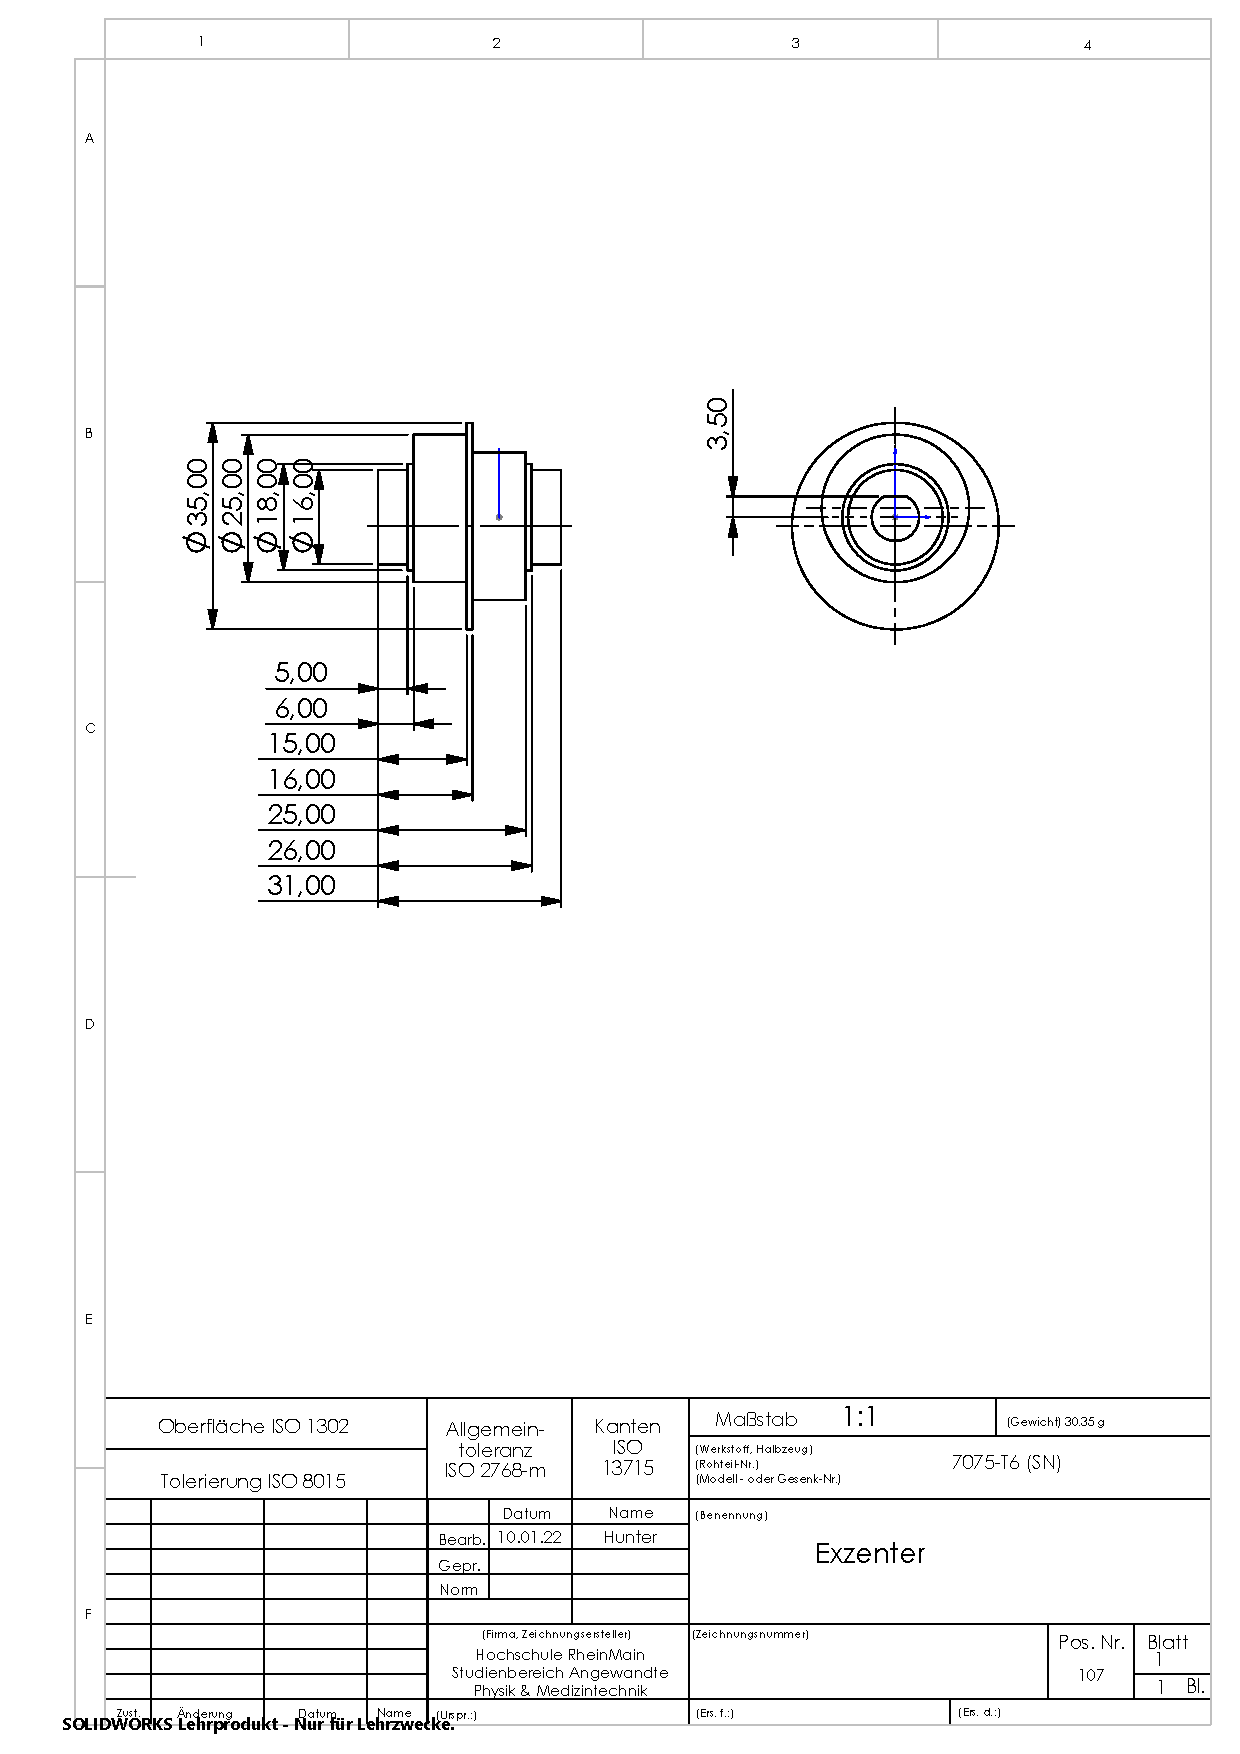
\includepdf[pages=-, angle=0, pagecommand={\thispagestyle{plain}}, addtolist={1, figure, Exzenter, drw:Exzenter}, addtotoc={1, section, 1, Einzelteilzeichnungen Schultergelenk, sec:einzelteilzeichnungen schultergelenk}]{Abb/CAD/Drawings/Schulter/Exzenter.pdf}
%
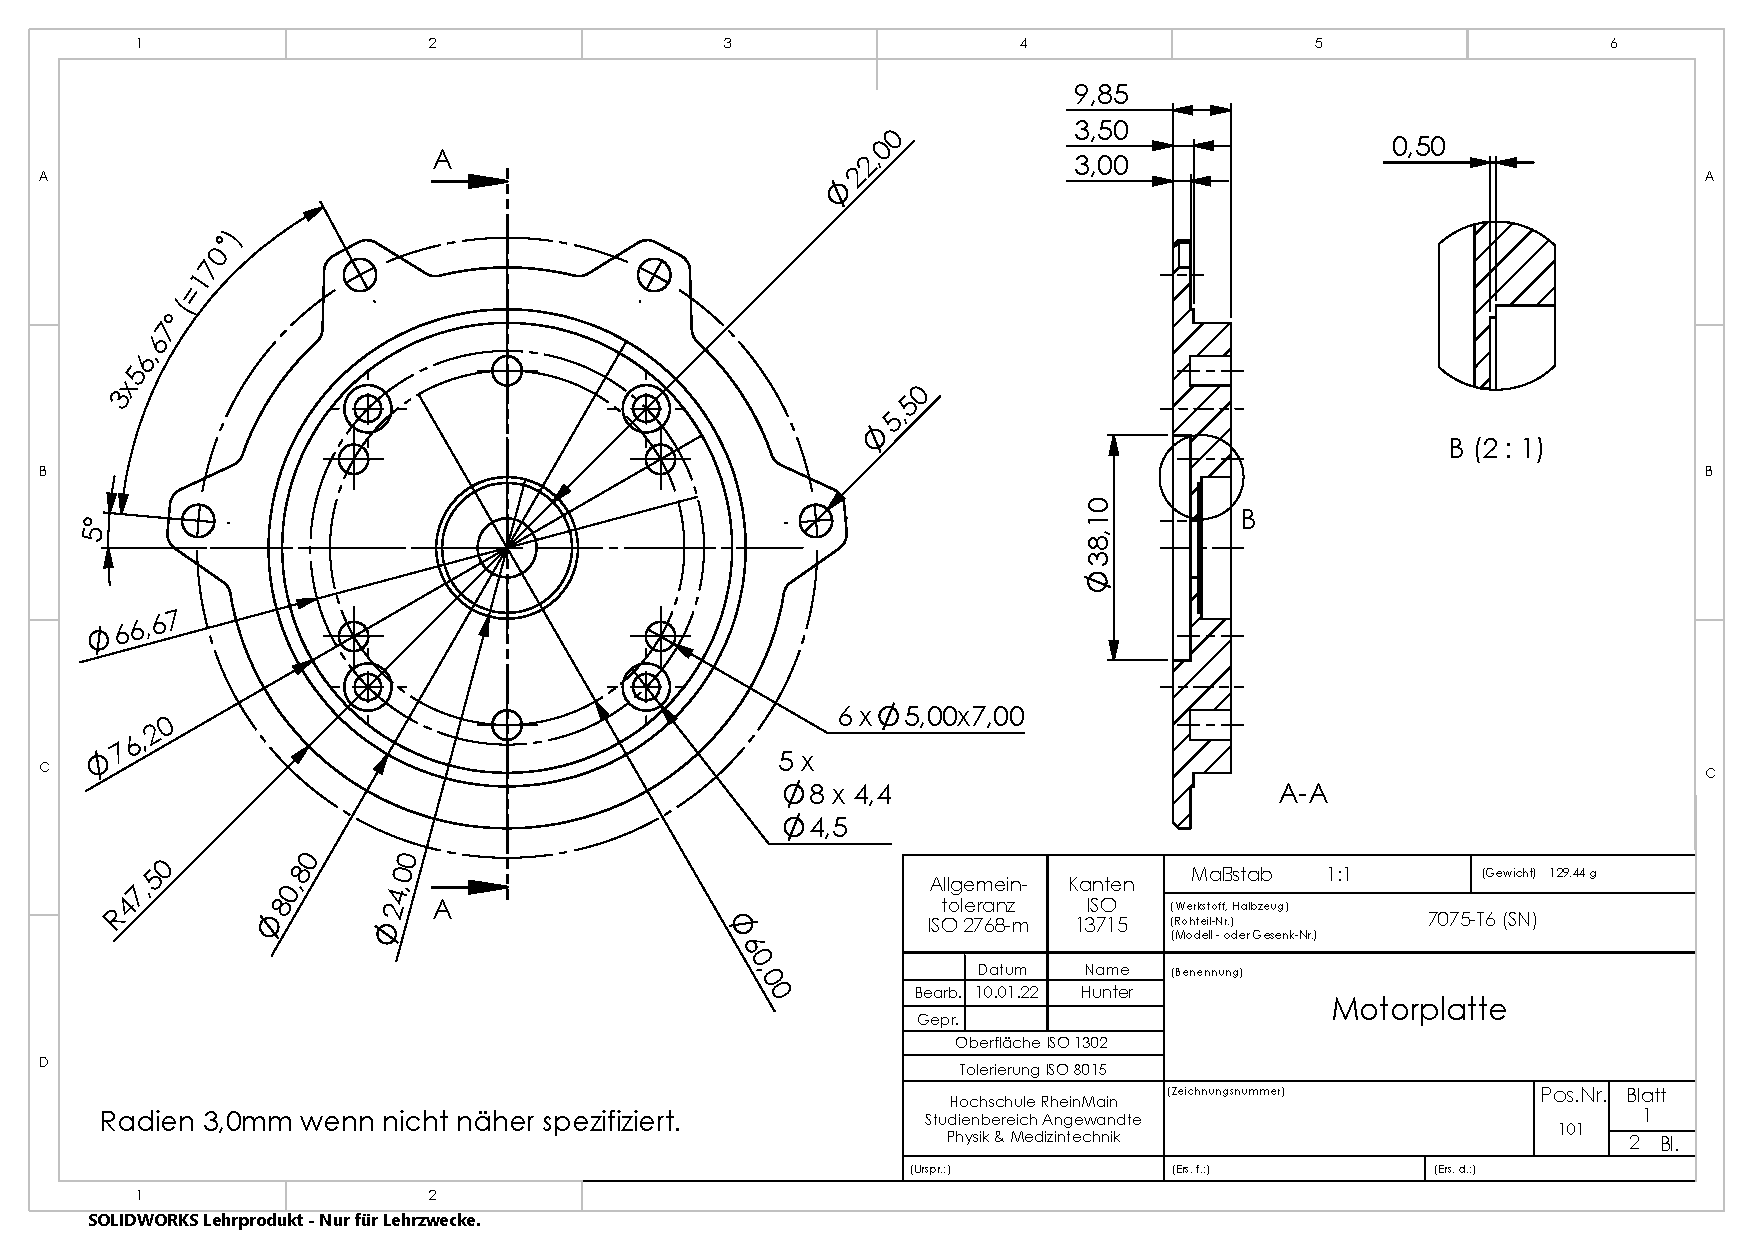
\includepdf[pages=-, angle=90, pagecommand={\thispagestyle{plain}}, addtolist={1, figure, Motor- und Fixierplatte, drw:Motor und Fixierplatte}]{Abb/CAD/Drawings/Schulter/Motorplatte-Fixierplatte.pdf}
%
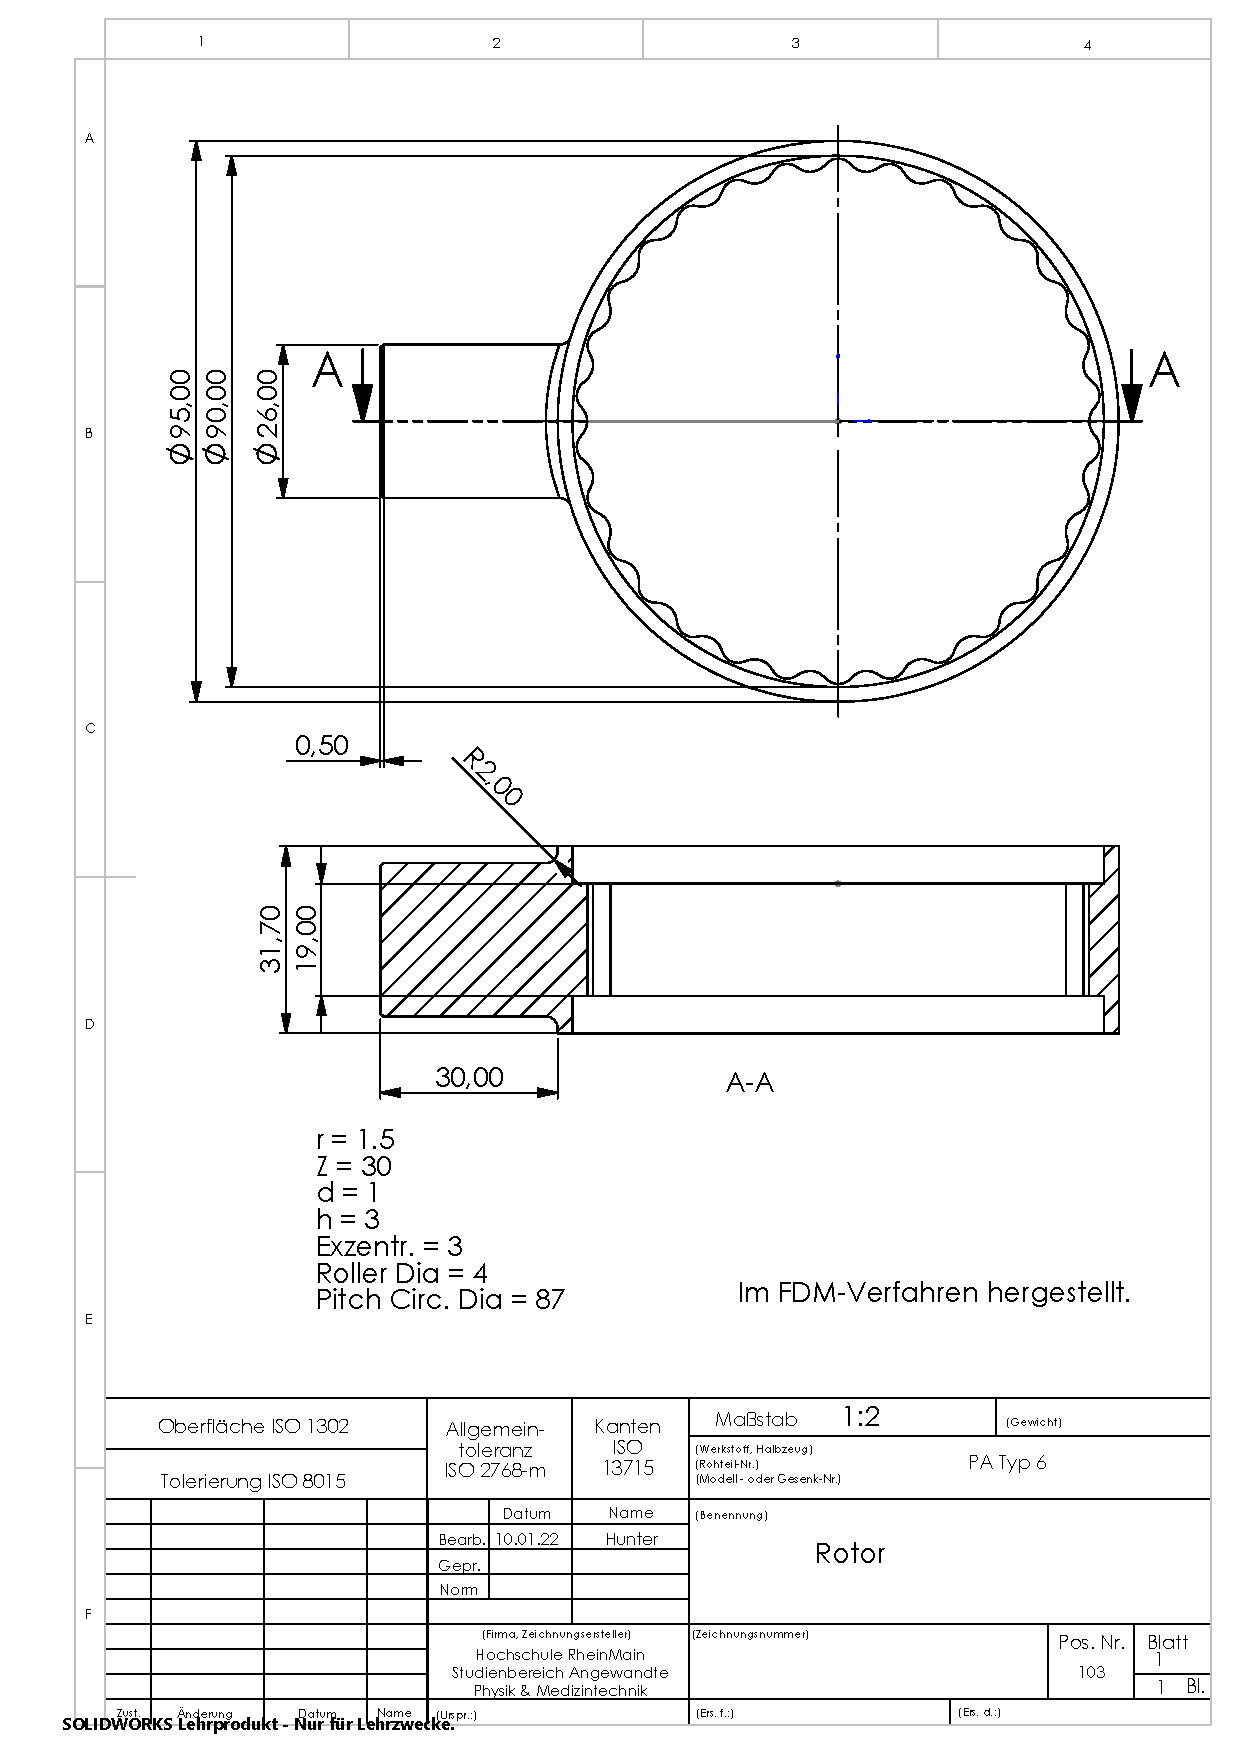
\includepdf[pages=-, angle=0, pagecommand={\thispagestyle{plain}}, addtolist={1, figure, Rotor, drw:Rotor}]{Abb/CAD/Drawings/Schulter/Rotor.pdf}
%
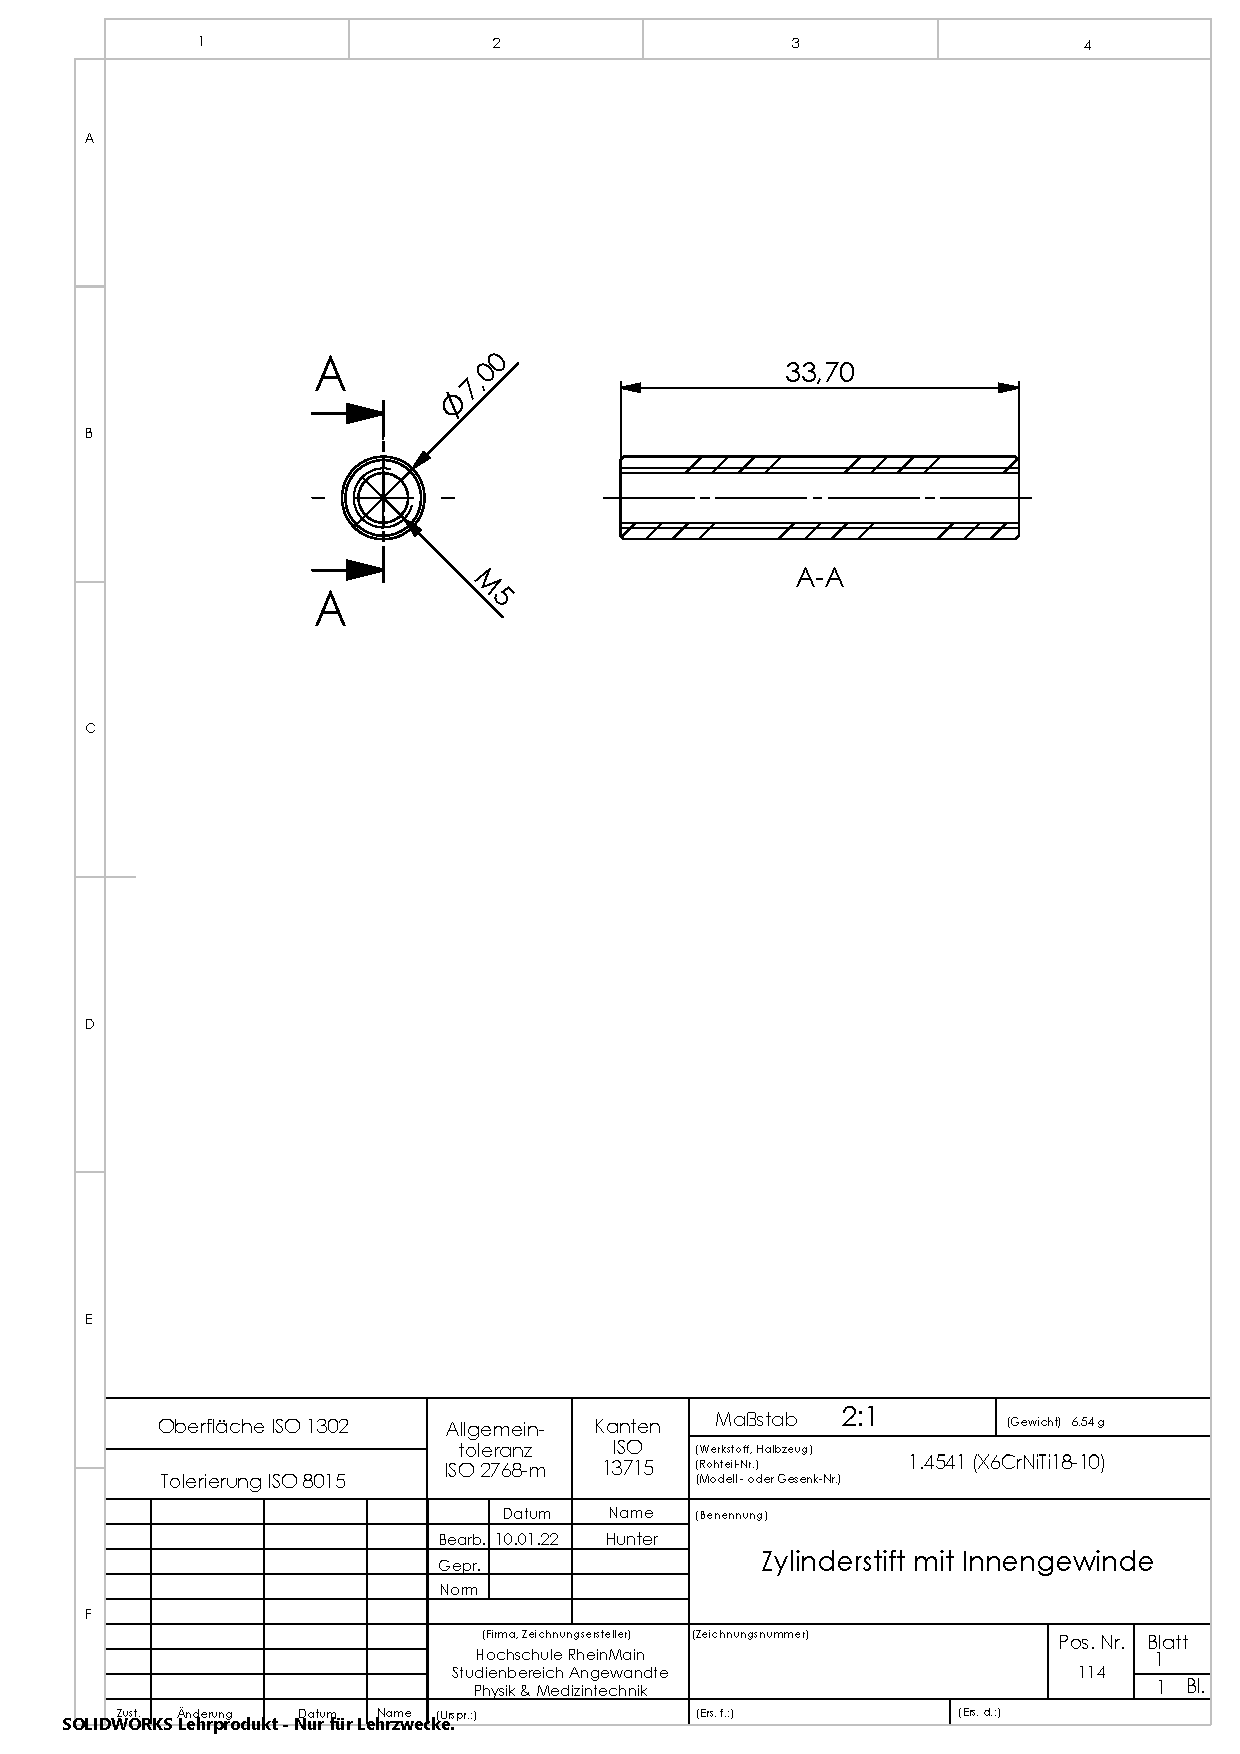
\includepdf[pages=-, angle=0, pagecommand={\thispagestyle{plain}}, addtolist={1, figure, Zylinderstift, drw:Zylinderstift}]{Abb/CAD/Drawings/Schulter/Zylinderstift-mit-Innengewinde.pdf}
%
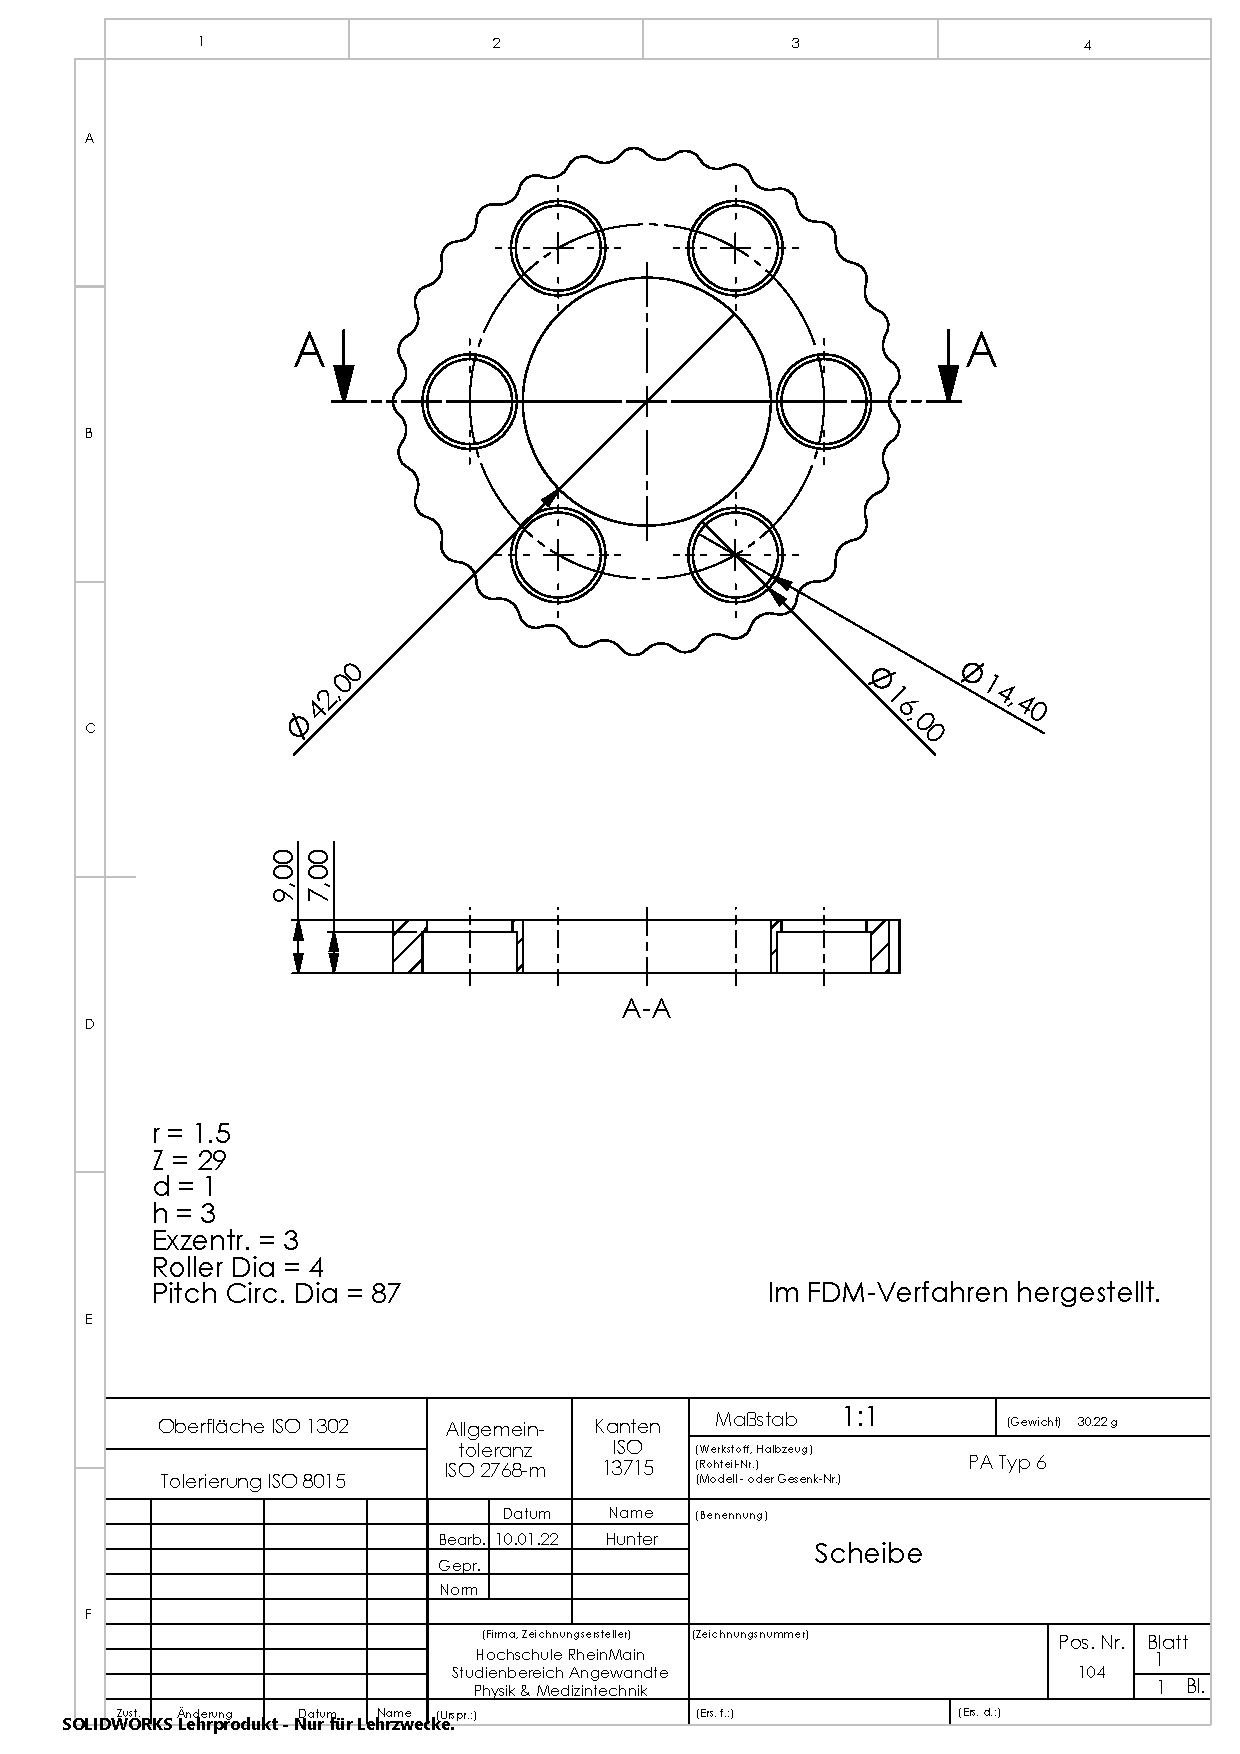
\includepdf[pages=-, angle=0, pagecommand={\thispagestyle{plain}}, addtolist={1, figure, Zahnscheibe, drw:Scheibe}]{Abb/CAD/Drawings/Schulter/Scheibe.pdf}
%
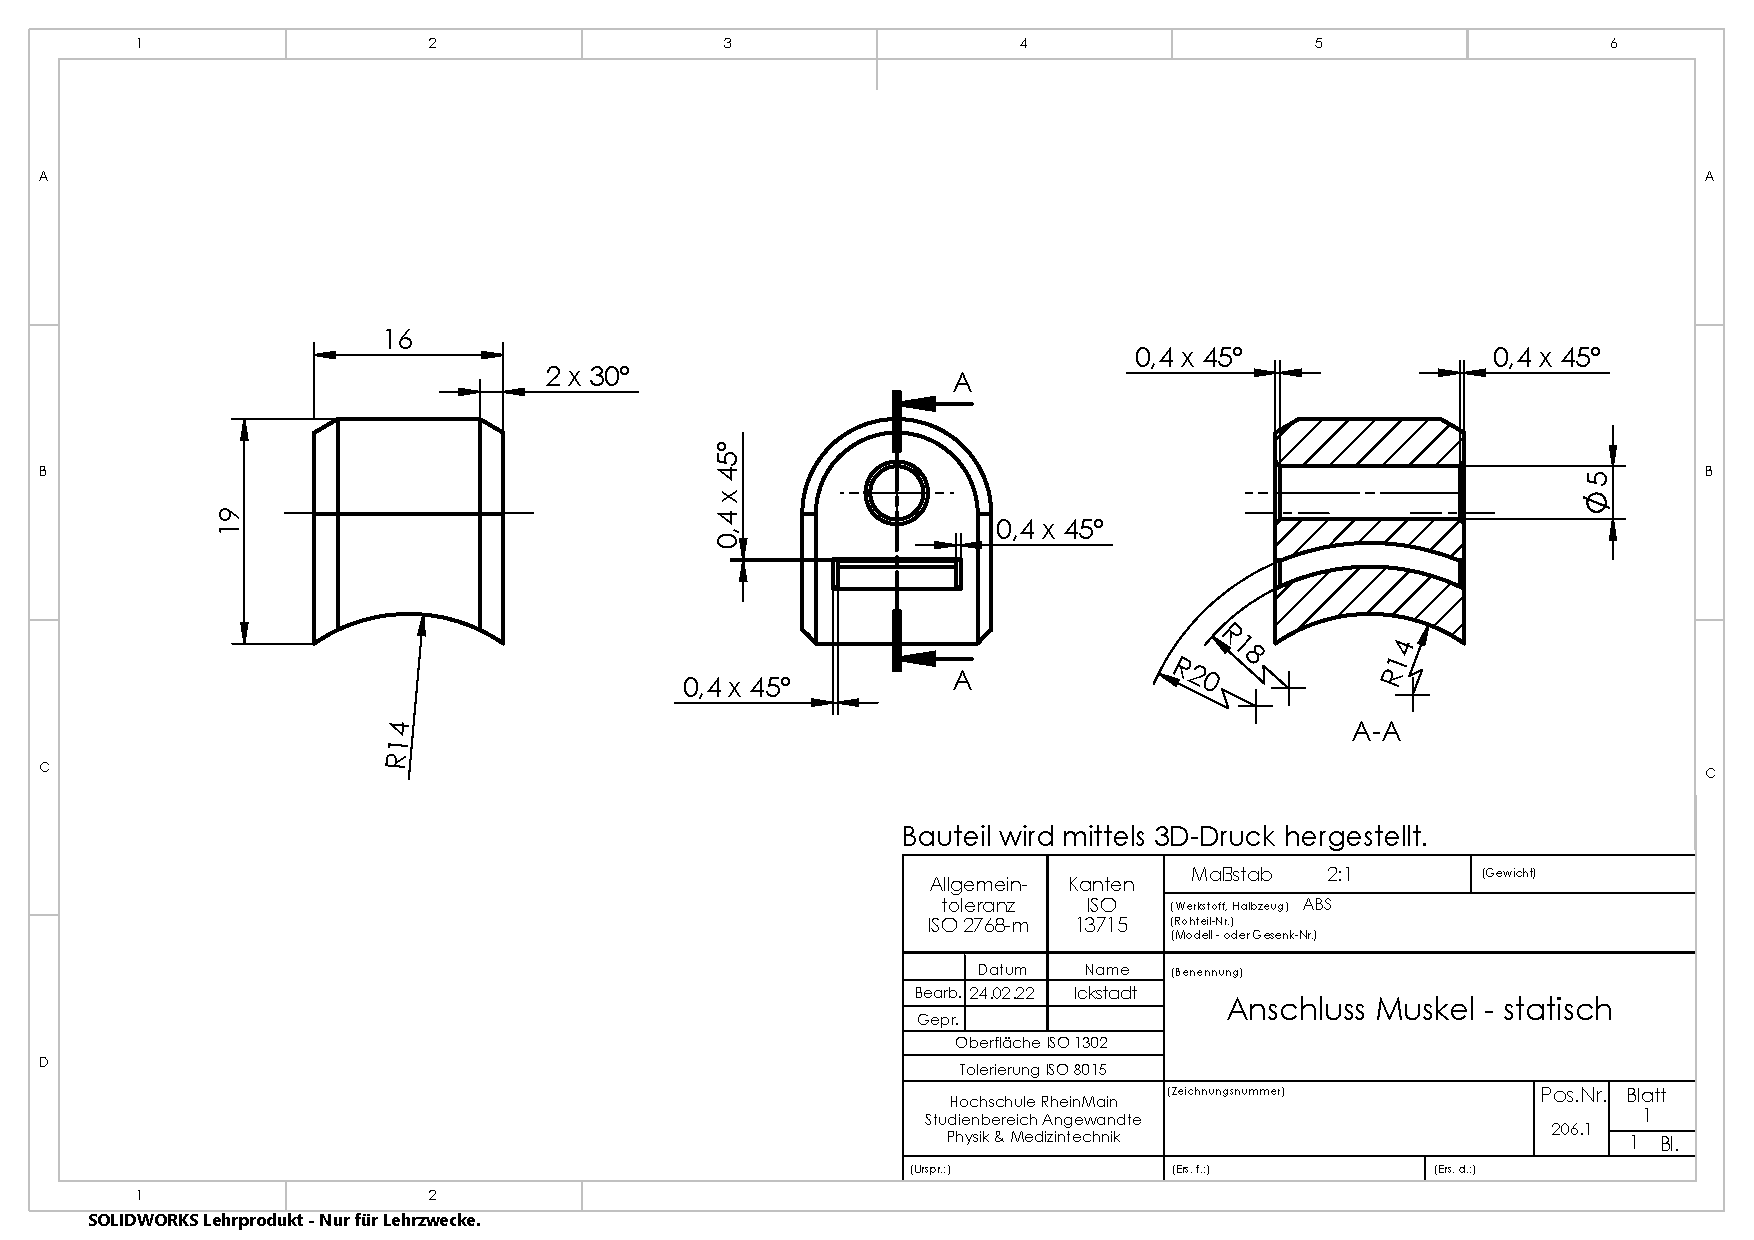
\includepdf[pages=-, angle=90, pagecommand={\thispagestyle{plain}}, addtolist={1, figure, Muskelanschluss, drw:Muskelanschluss}, addtotoc={1, section, 1, Einzelteilzeichnungen Arme, sec:einzelteilzeichnungen arme}]{Abb/CAD/Drawings/Anschluss-Muskel-statisch.pdf}
%
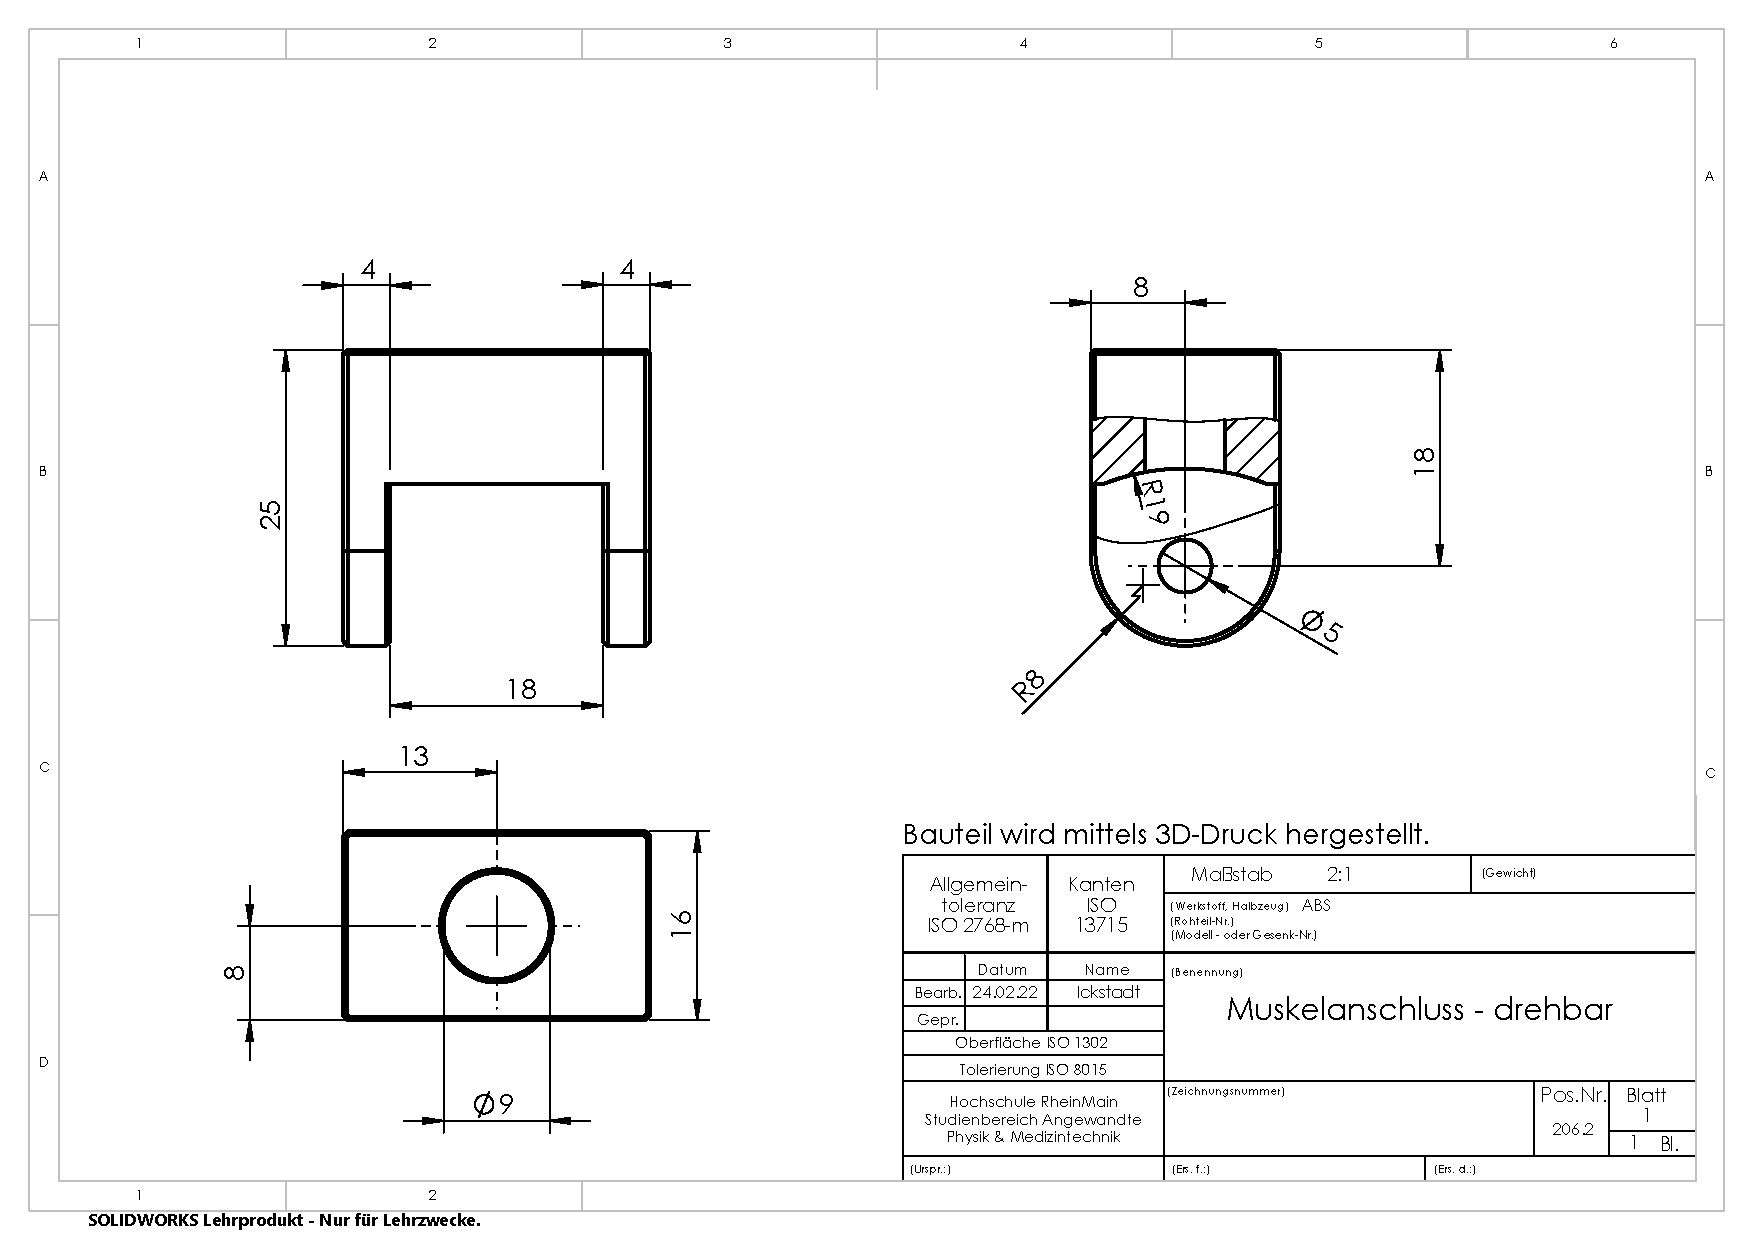
\includepdf[pages=-, angle=90, pagecommand={\thispagestyle{plain}}, addtolist={1, figure, Muskelanschluss drehbar, drw:Muskelanschluss-drehbar}]{Abb/CAD/Drawings/Muskelanschluss-drehbar.pdf}
%
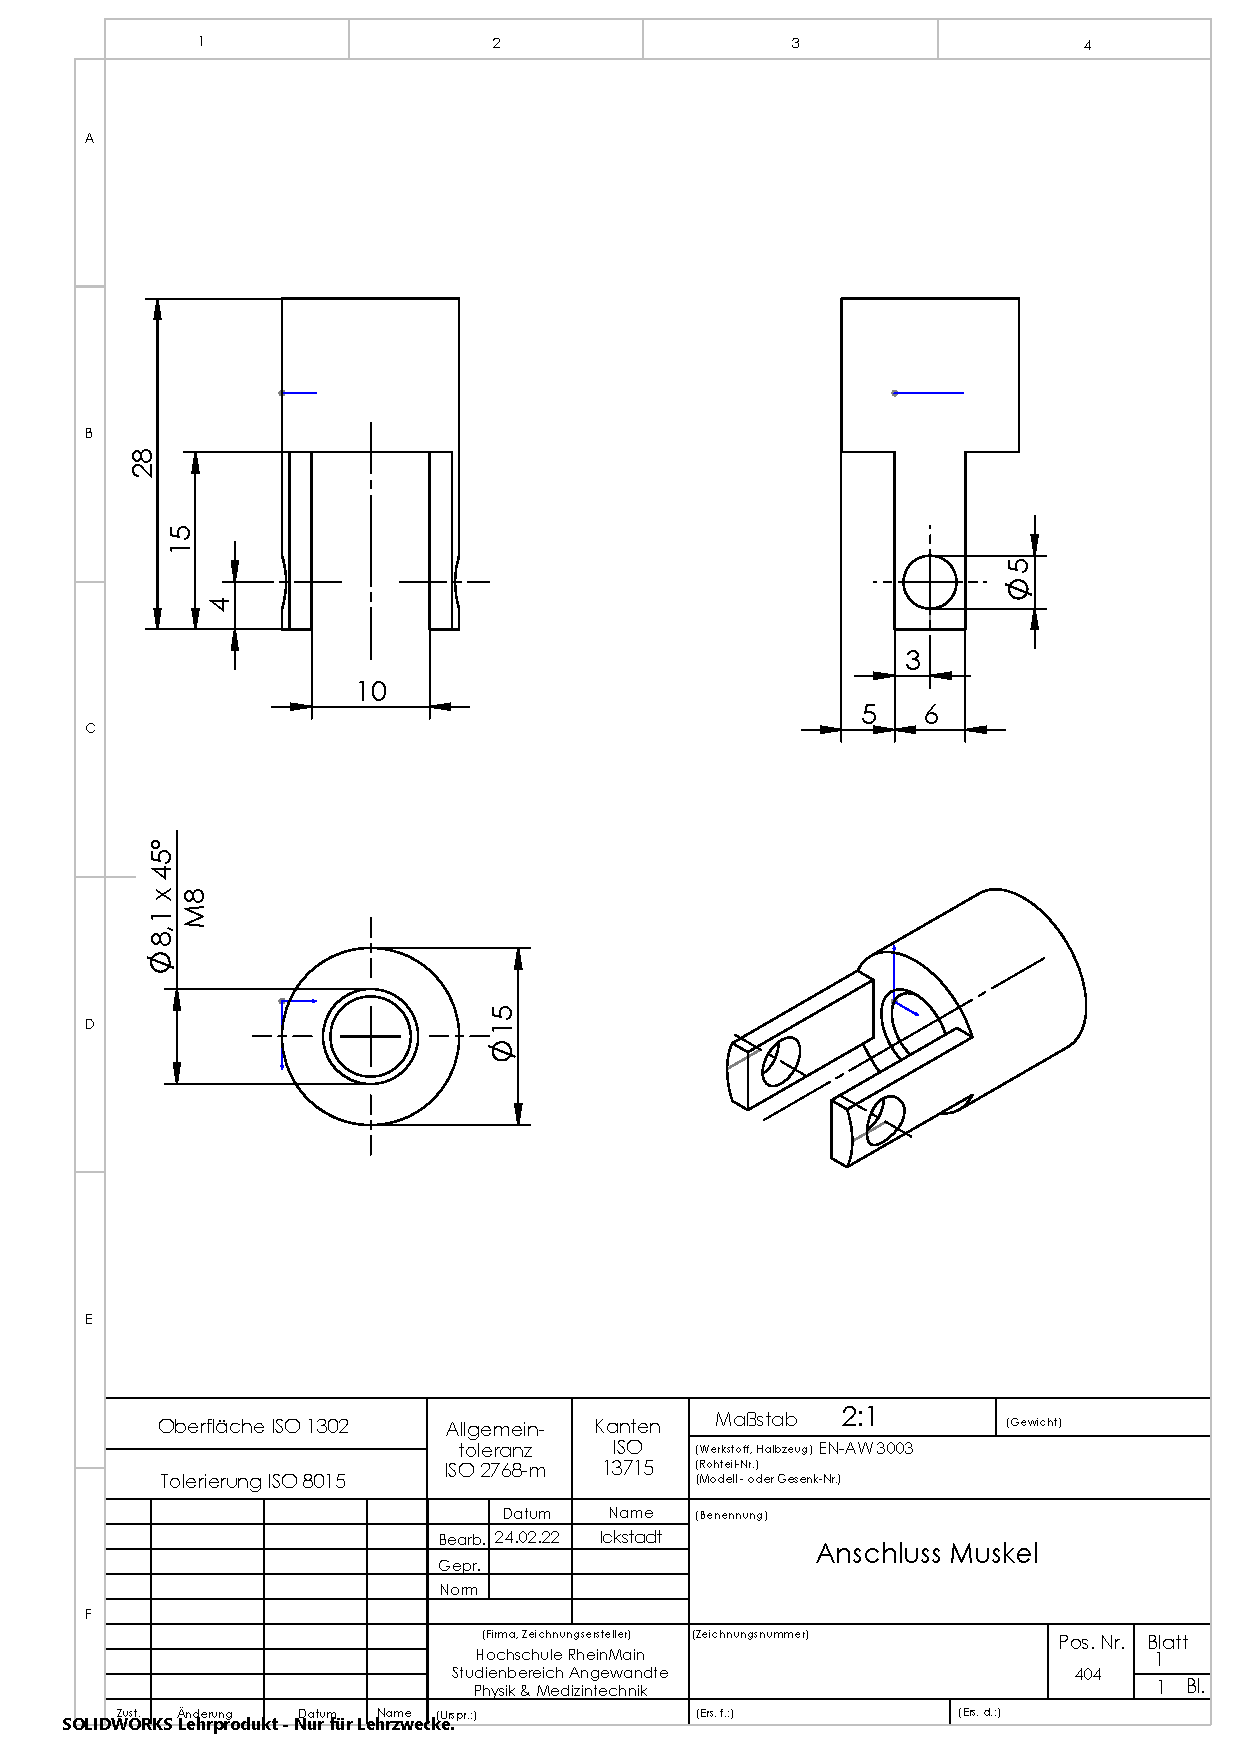
\includepdf[pages=-, angle=0, pagecommand={\thispagestyle{plain}}, addtolist={1, figure, Anschluss-Muskel, drw:Anschluss-Muskel}]{Abb/CAD/Drawings/Anschluss-Muskel.pdf}
%
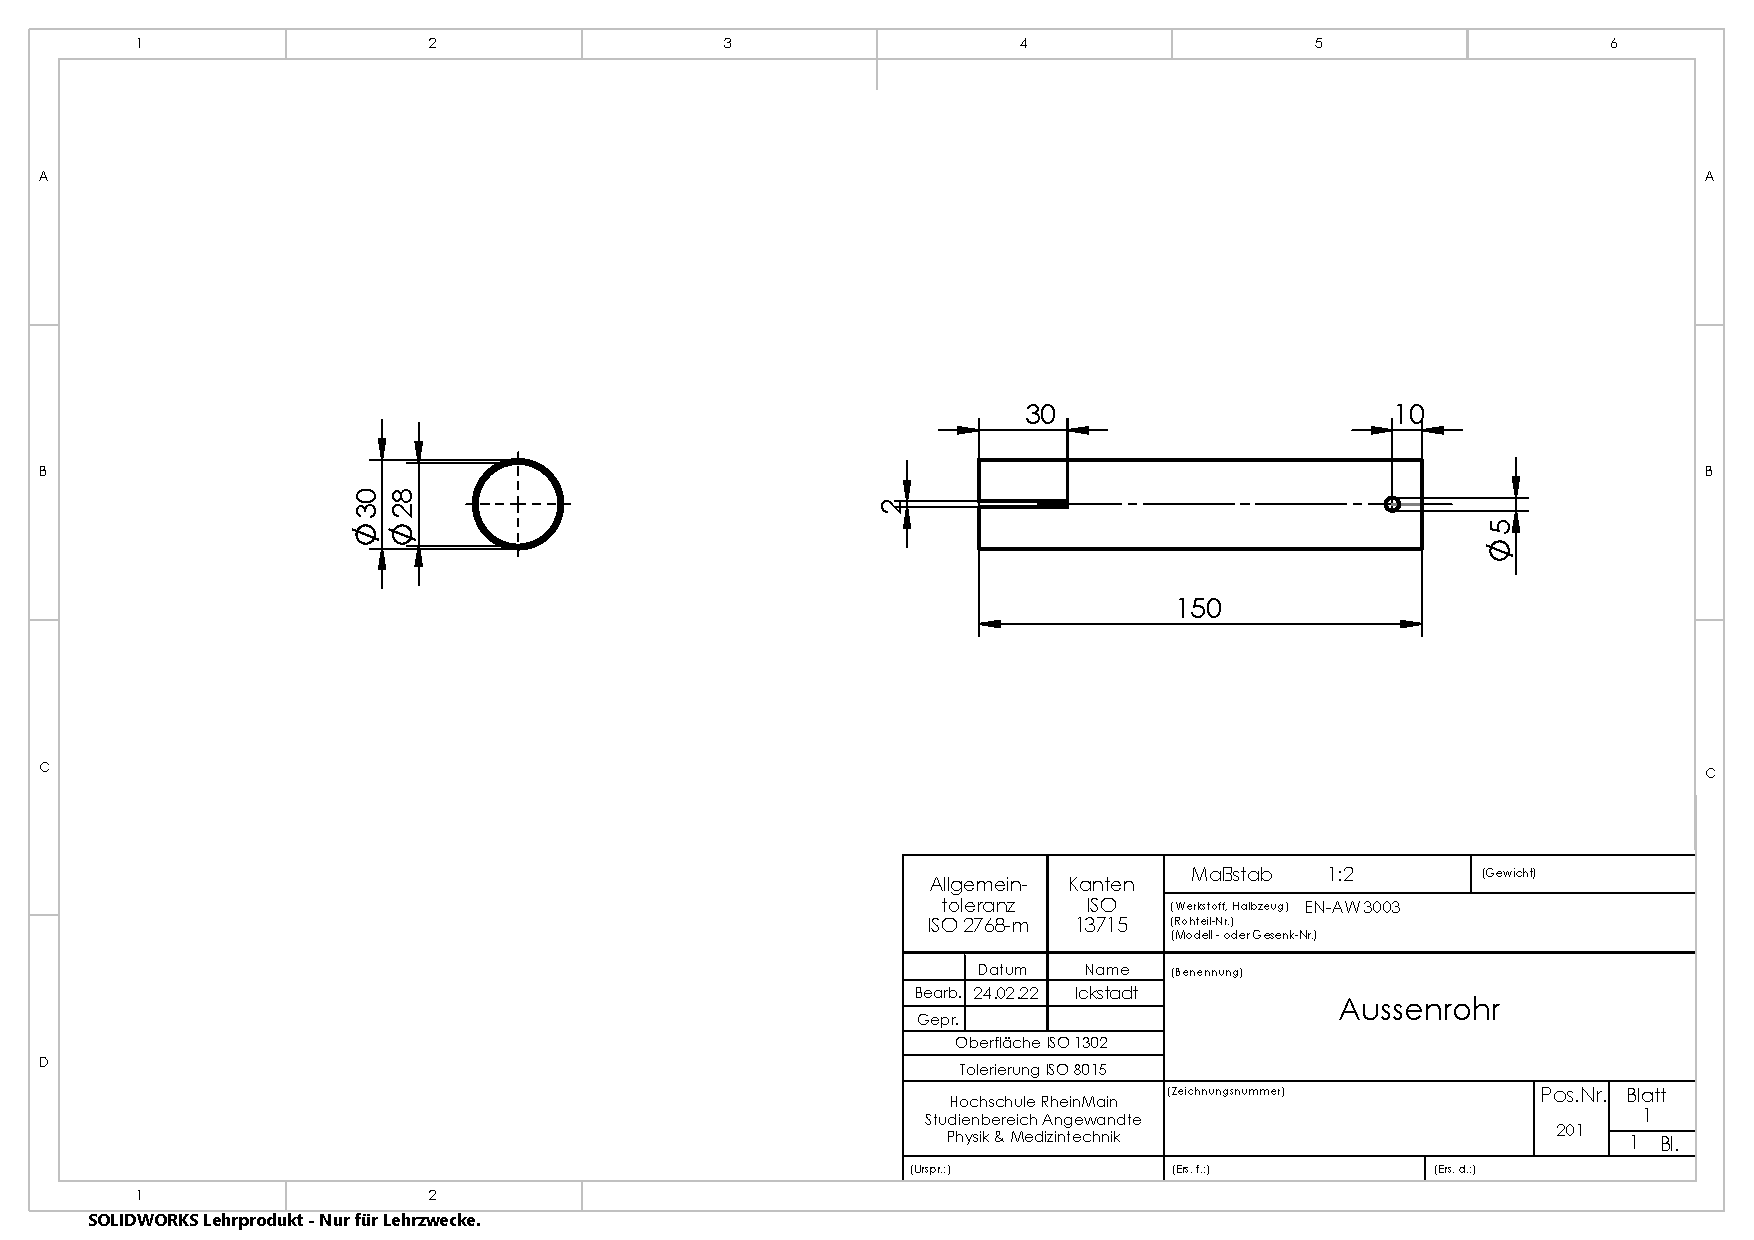
\includepdf[pages=-, angle=90, pagecommand={\thispagestyle{plain}}, addtolist={1, figure, Aussenrohr, drw:Aussenrohr}]{Abb/CAD/Drawings/Aussenrohr.pdf}
%
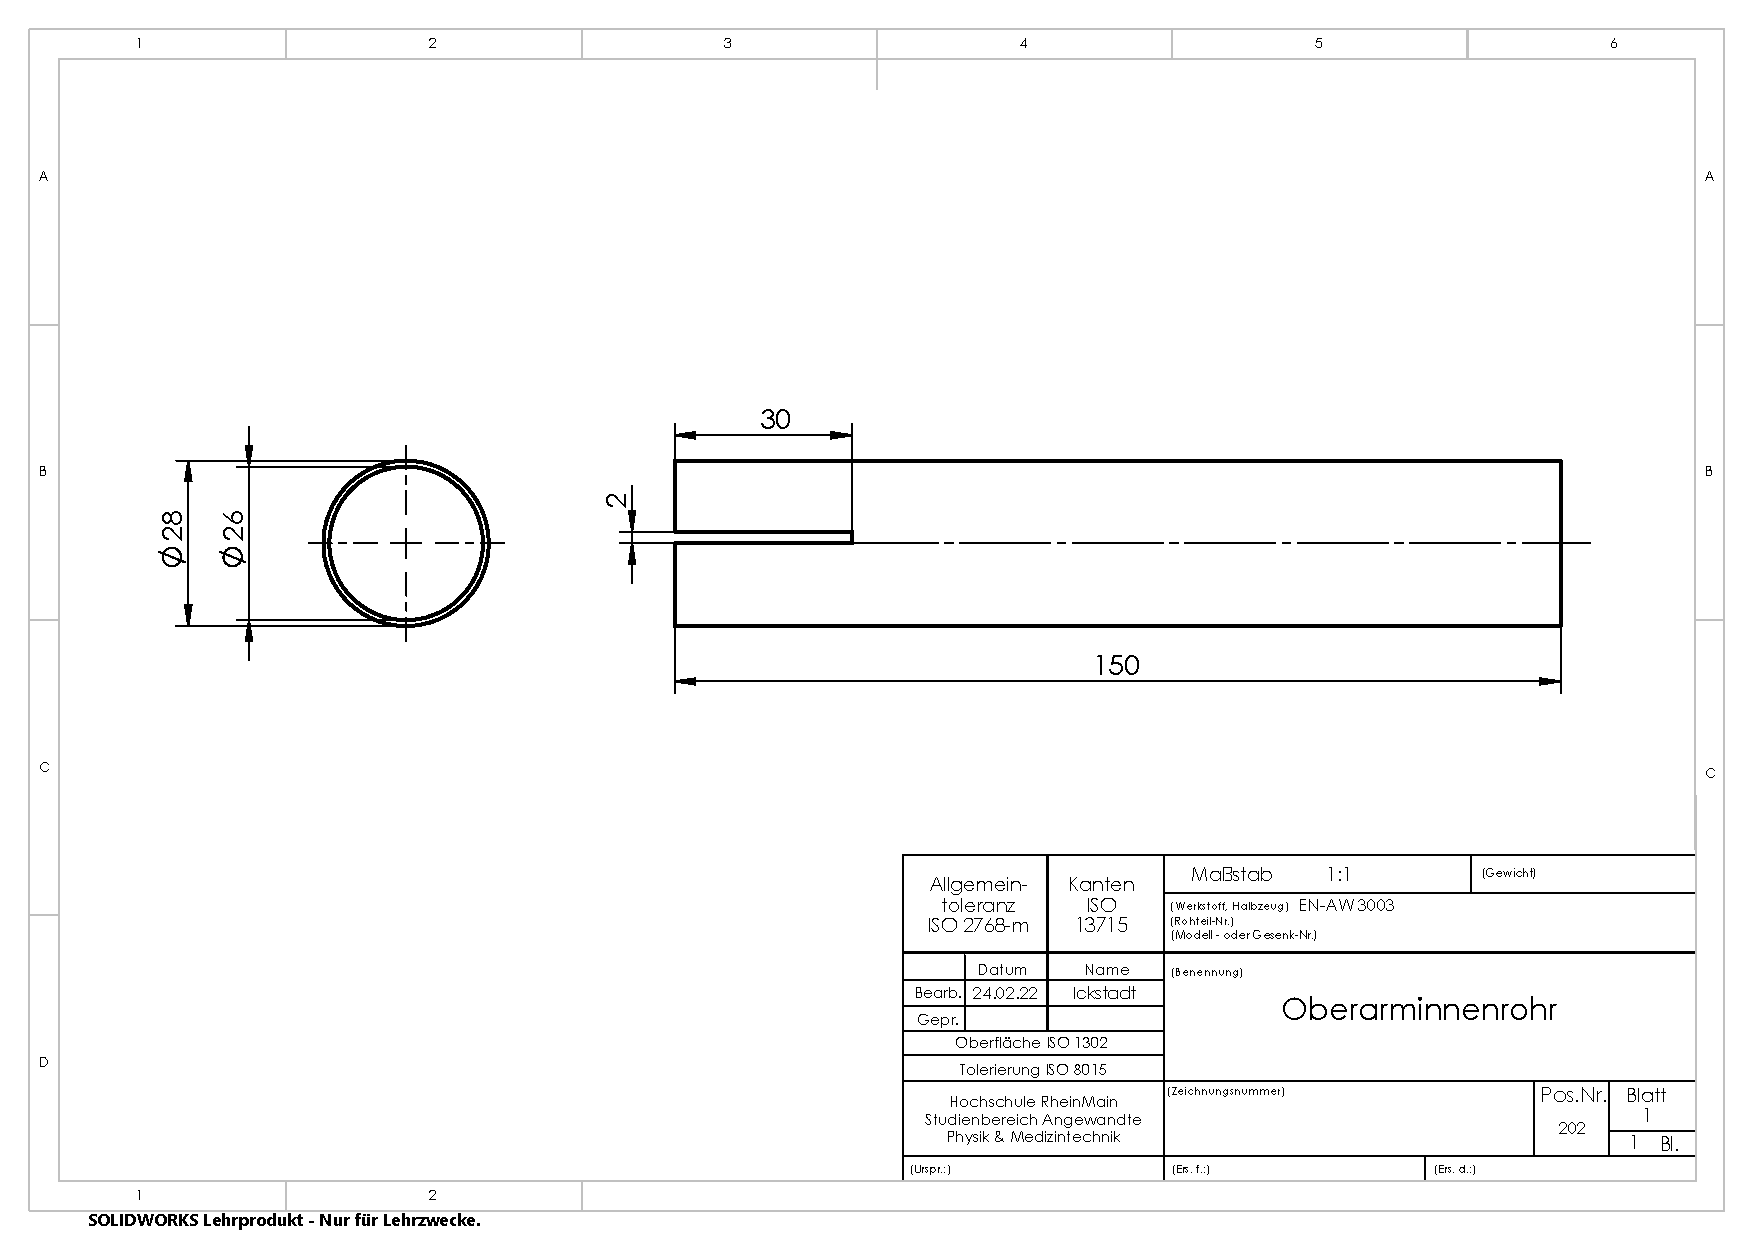
\includepdf[pages=-, angle=90, pagecommand={\thispagestyle{plain}}, addtolist={1, figure, Oberarminnenrohr, drw:Oberarminnenrohr}]{Abb/CAD/Drawings/Oberarminnenrohr.pdf}
%
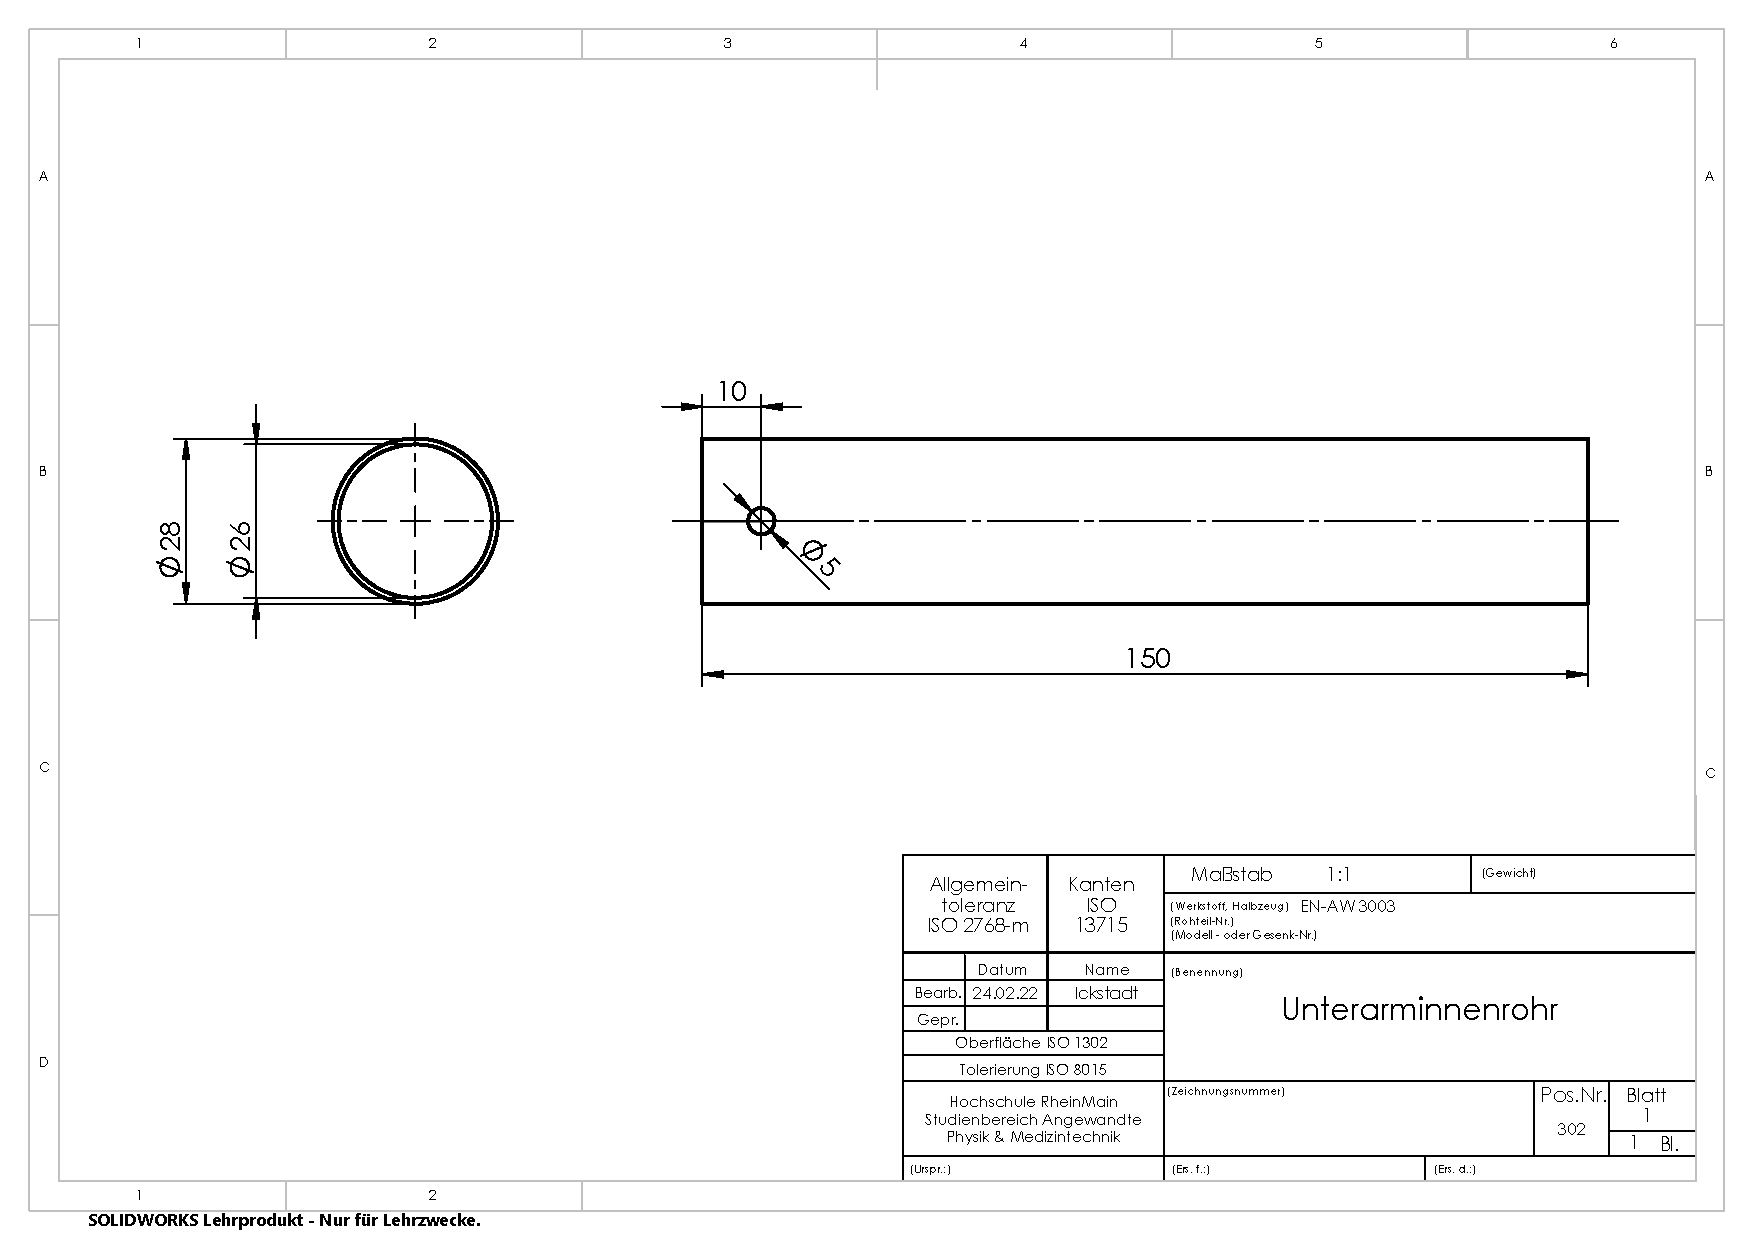
\includepdf[pages=-, angle=90, pagecommand={\thispagestyle{plain}}, addtolist={1, figure, Unterarminnenrohr, drw:Unterarminnenrohr}]{Abb/CAD/Drawings/Unterarminnenrohr.pdf}
%
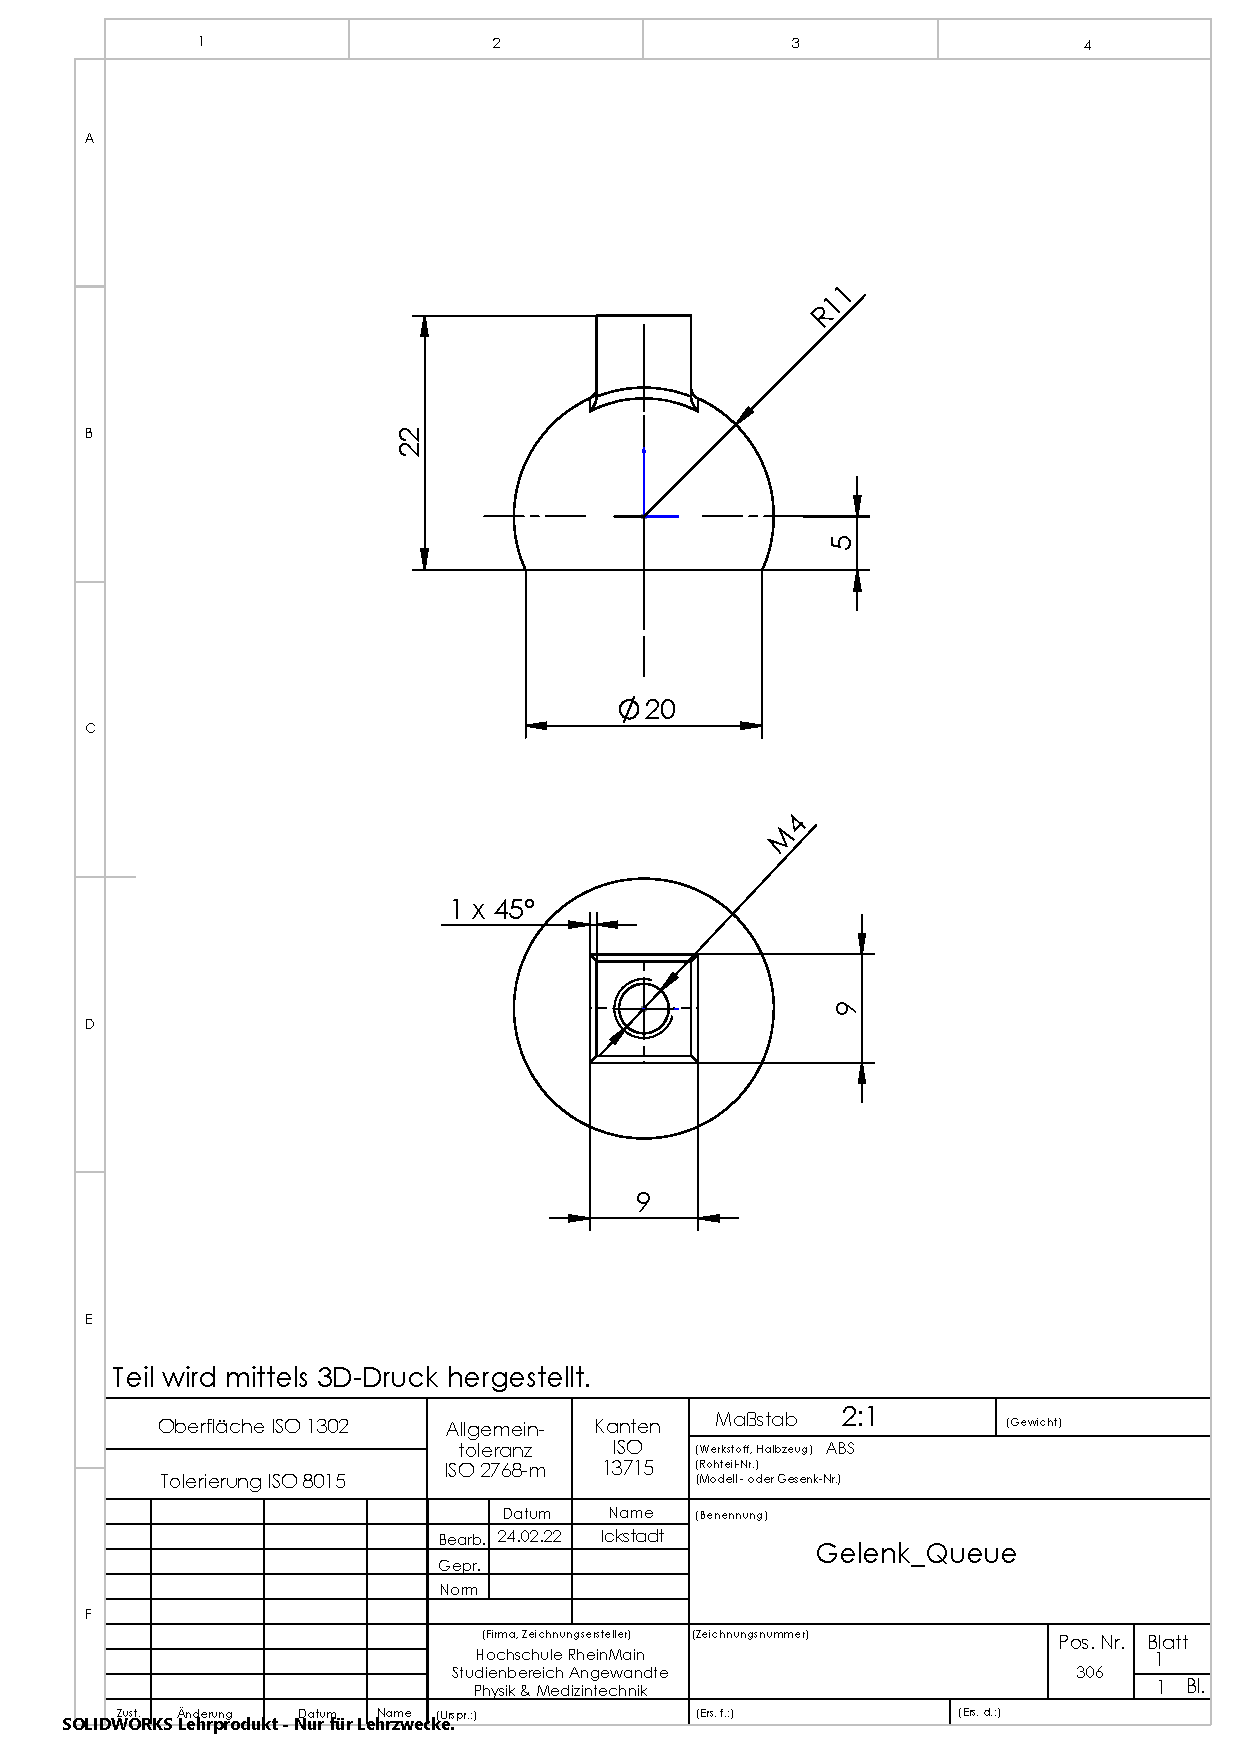
\includepdf[pages=-, angle=0, pagecommand={\thispagestyle{plain}}, addtolist={1, figure, Gelenk-Queue, drw:Gelenk-Queue}]{Abb/CAD/Drawings/Gelenk-Queue.pdf}
%
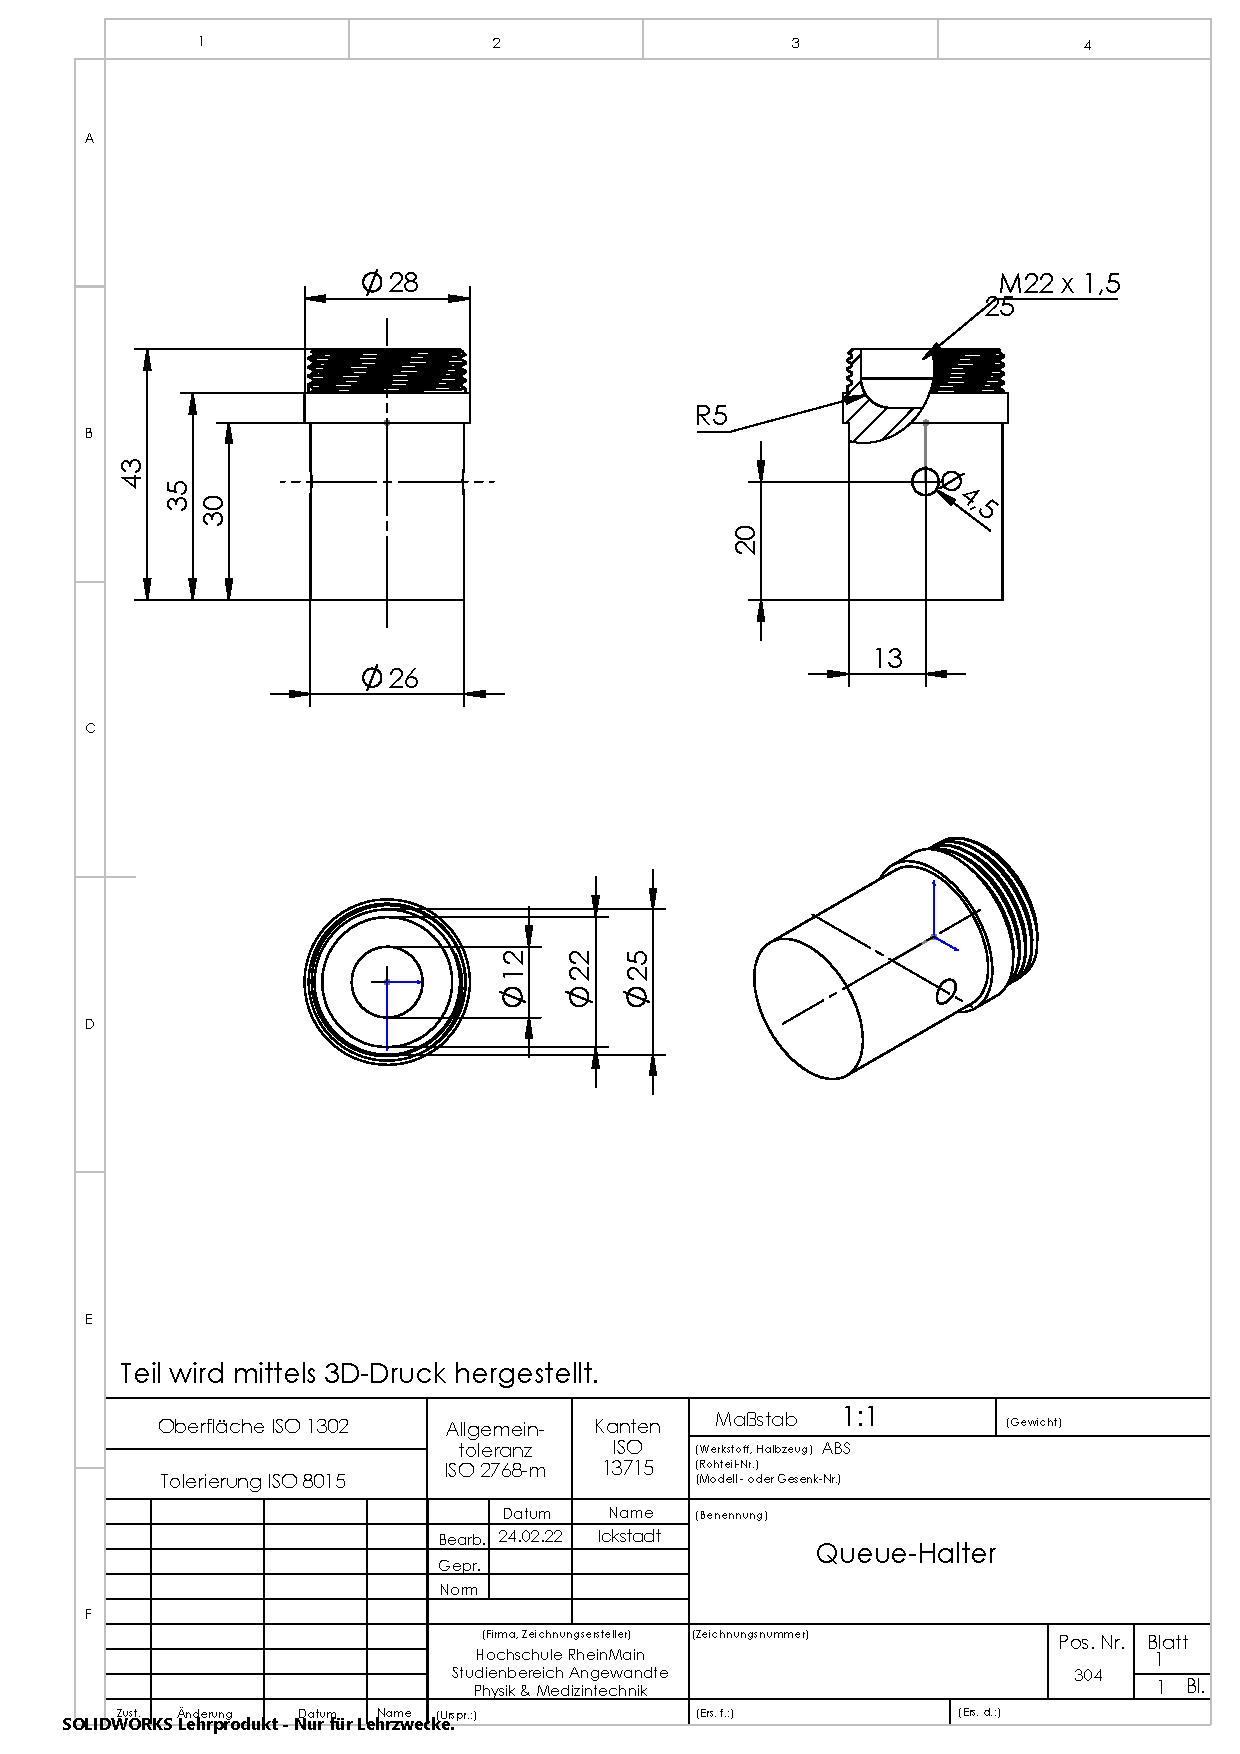
\includepdf[pages=-, angle=0, pagecommand={\thispagestyle{plain}}, addtolist={1, figure, Queue-Halter, drw:Queue-Halter}]{Abb/CAD/Drawings/Queue-Halter.pdf}
%
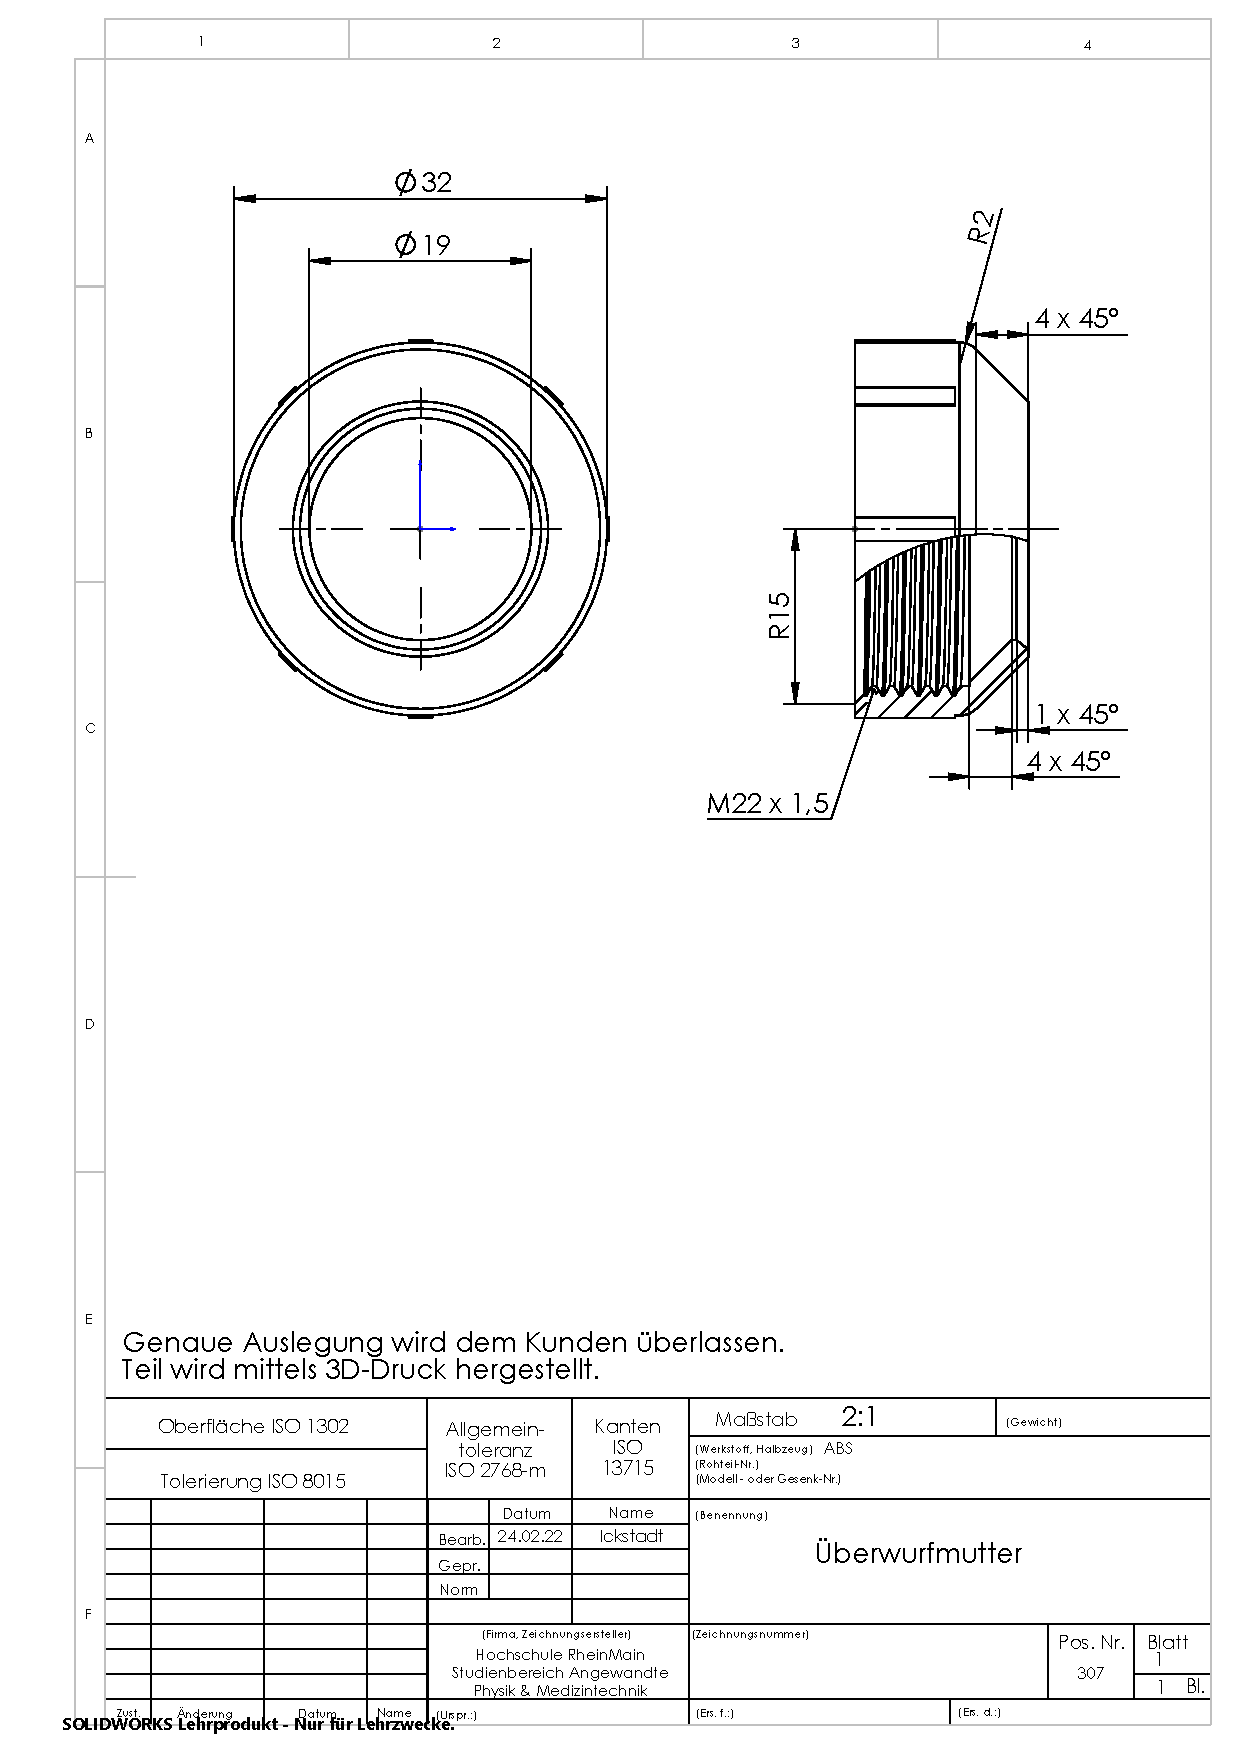
\includepdf[pages=-, angle=0, pagecommand={\thispagestyle{plain}}, addtolist={1, figure, Überwurfmutter, drw:Ueberwurfmutter}]{Abb/CAD/Drawings/Ueberwurfmutter.pdf}
%
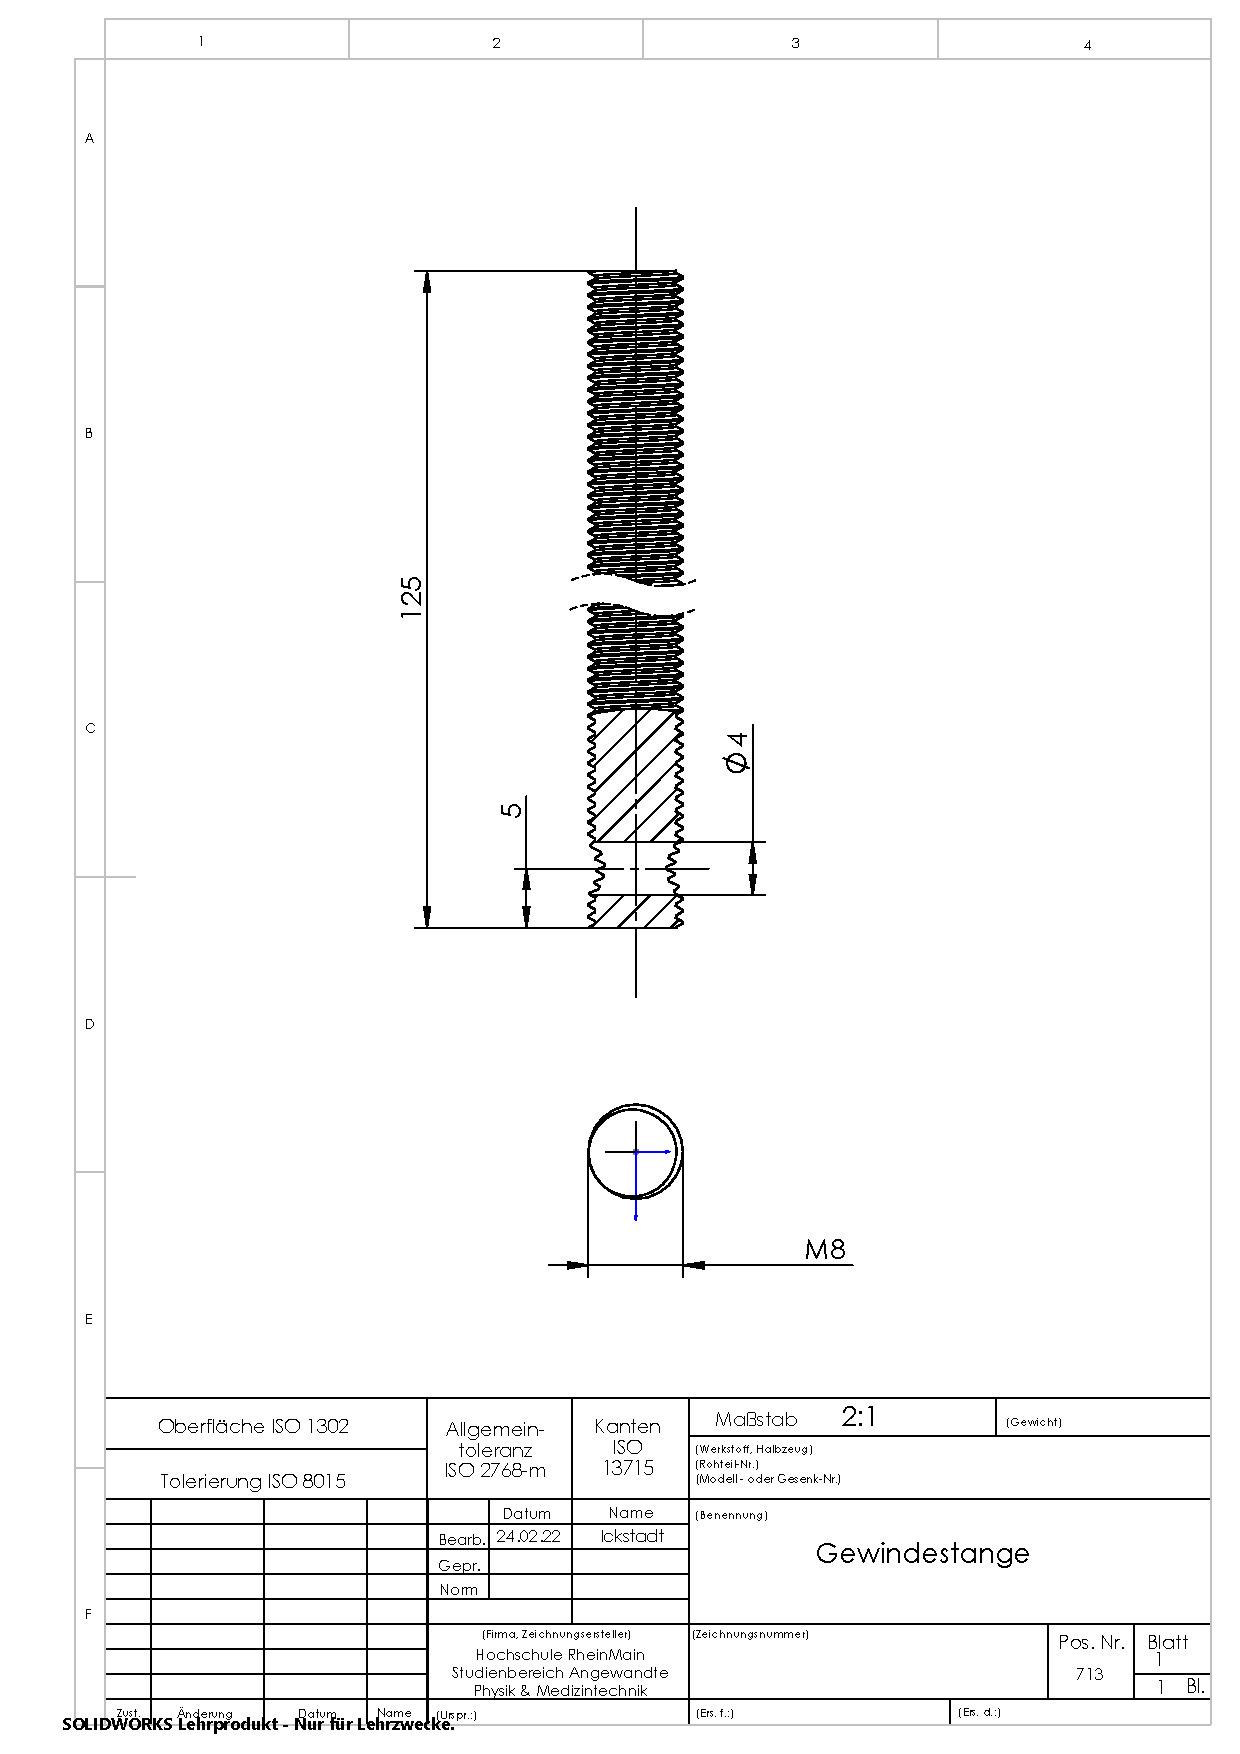
\includepdf[pages=-, angle=0, pagecommand={\thispagestyle{plain}}, addtolist={1, figure, Gewindestange, drw:Gewindestange}, addtotoc={1, section, 1, Einzelteilzeichnungen Ellbogengelenk, sec:einzelteilzeichnungen ellbogengelenk}]{Abb/CAD/Drawings/Gewindestange.pdf}
%
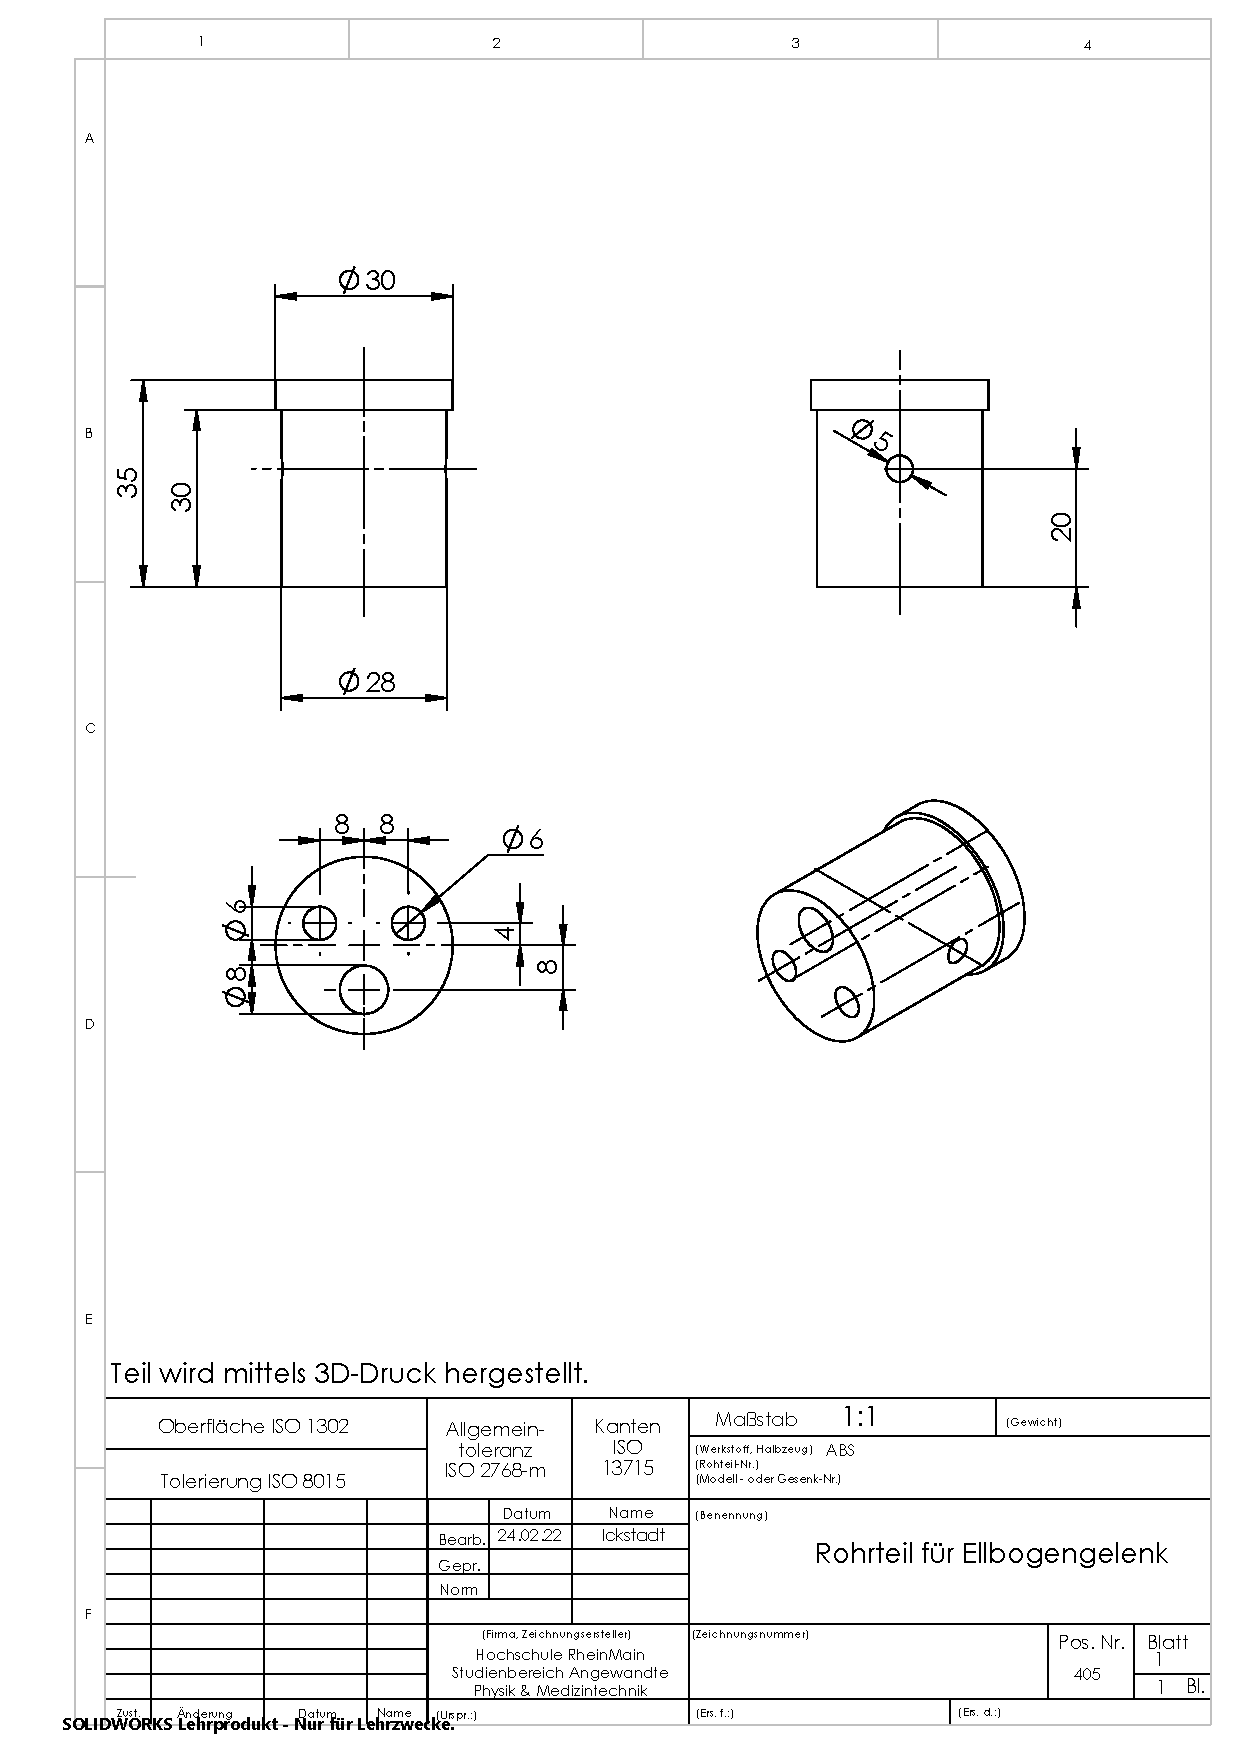
\includepdf[pages=-, angle=0, pagecommand={\thispagestyle{plain}}, addtolist={1, figure, Rohrteil für Ellbogengelenk, drw:Rohrteil-fuer-Ellbogengelenk}]{Abb/CAD/Drawings/Rohrteil-fuer-Ellbogengelenk.pdf}
%
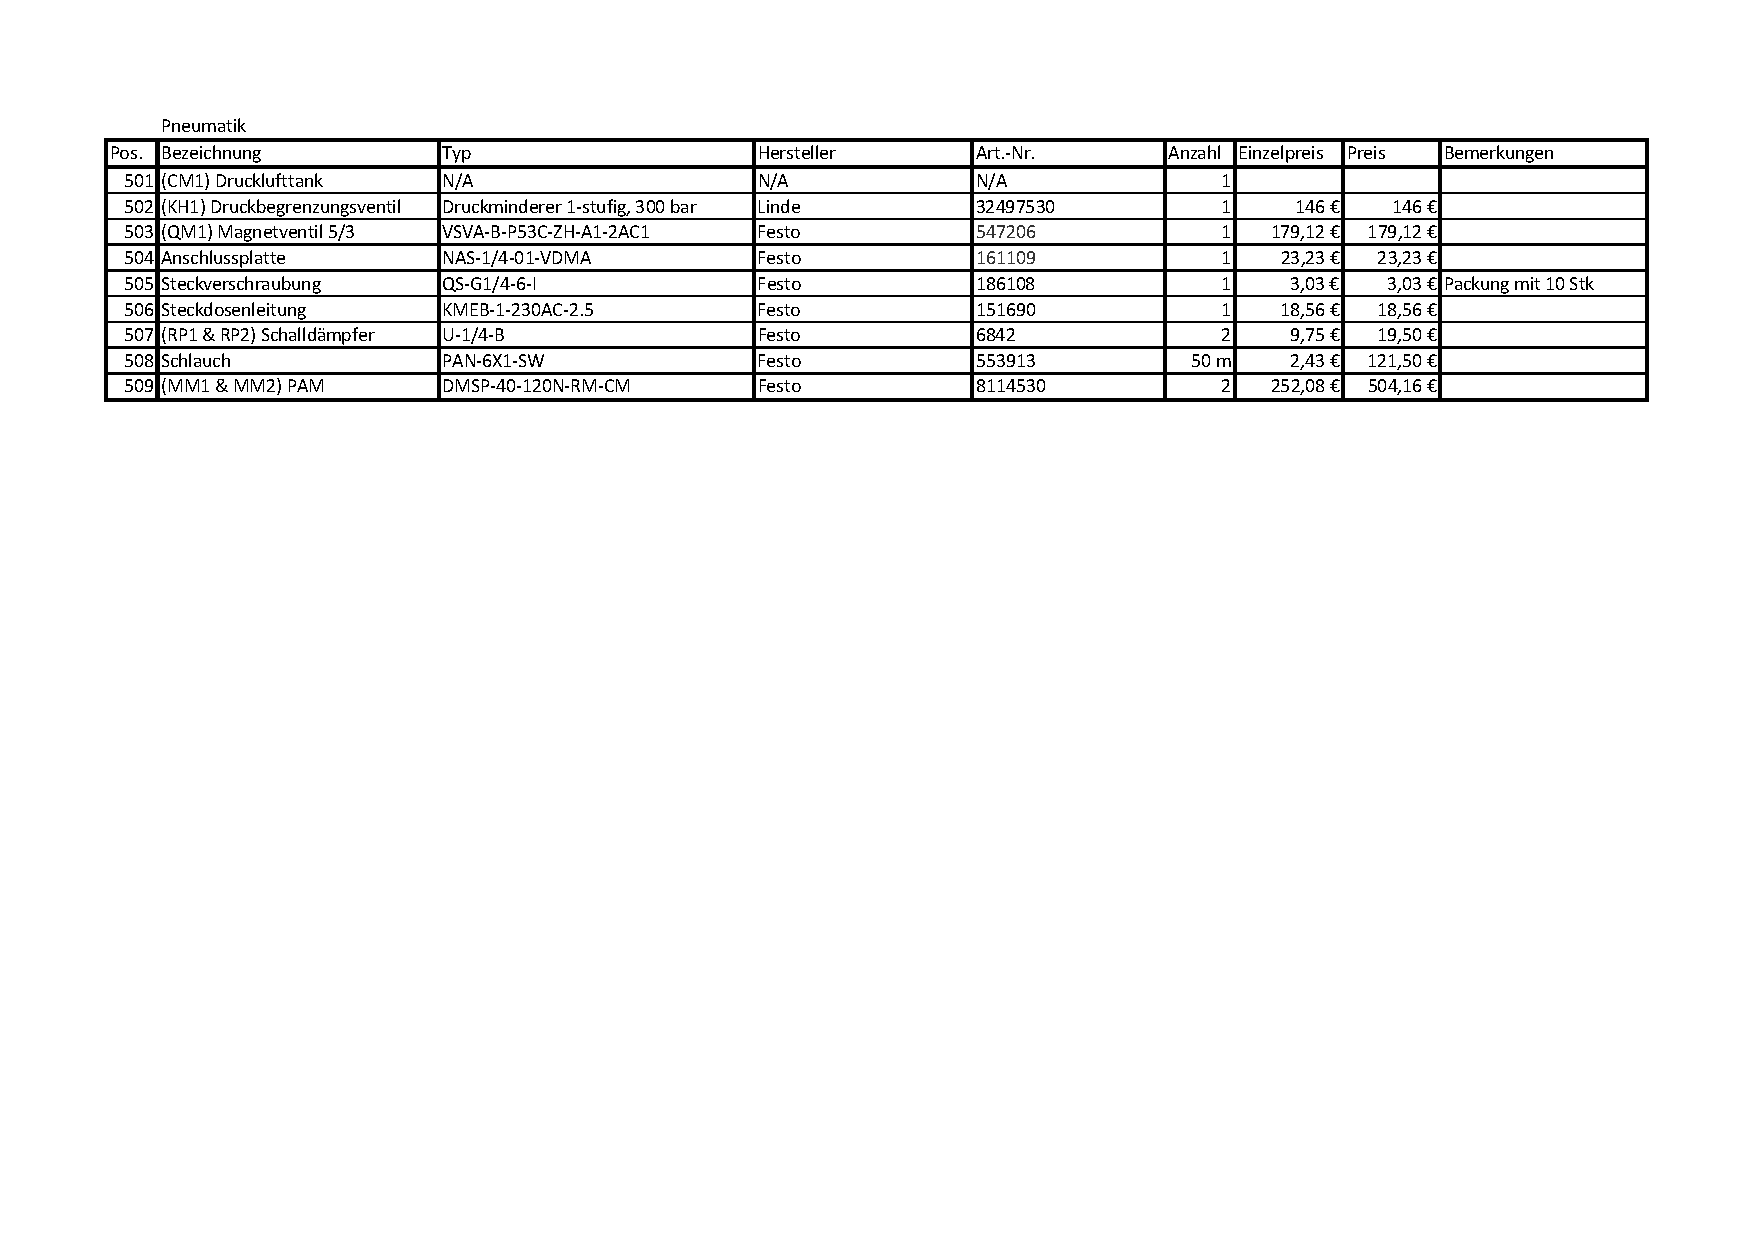
\includepdf[pages=-, angle=90, pagecommand={\thispagestyle{plain}}, addtolist={1, table, Stückliste Pneumatik, tab:StuecklistePneumatik}, addtotoc={1, section, 1, Generelle Stückliste und Pneumatikschaltplan, sec:stueckliste und pneumatikschaltplan}]{Abb/Stuecklisten/StuecklistePneumatik.pdf}
%
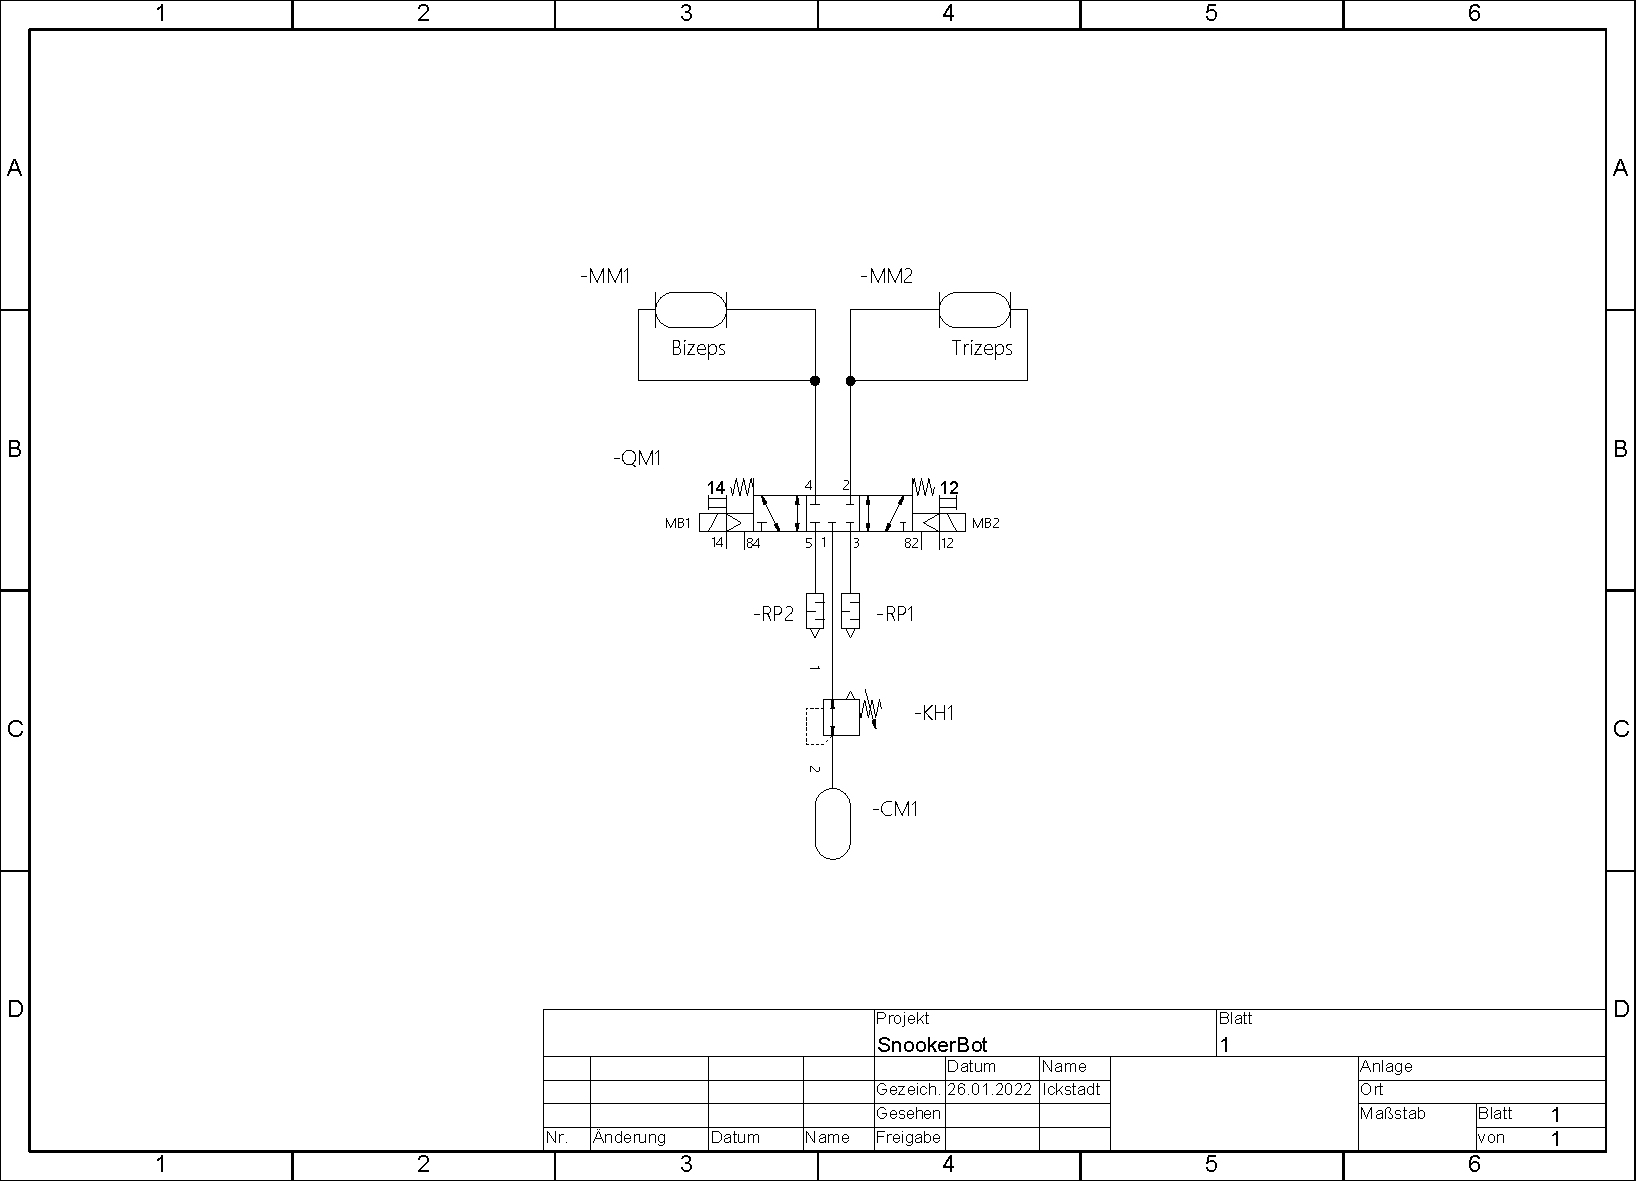
\includepdf[pages=-, angle=90, pagecommand={\thispagestyle{plain}}, addtolist={1, figure, Pneumatikschaltplan, drw:PneumatikZeichnung}]{Abb/PneumatikZeichnung.pdf}
%
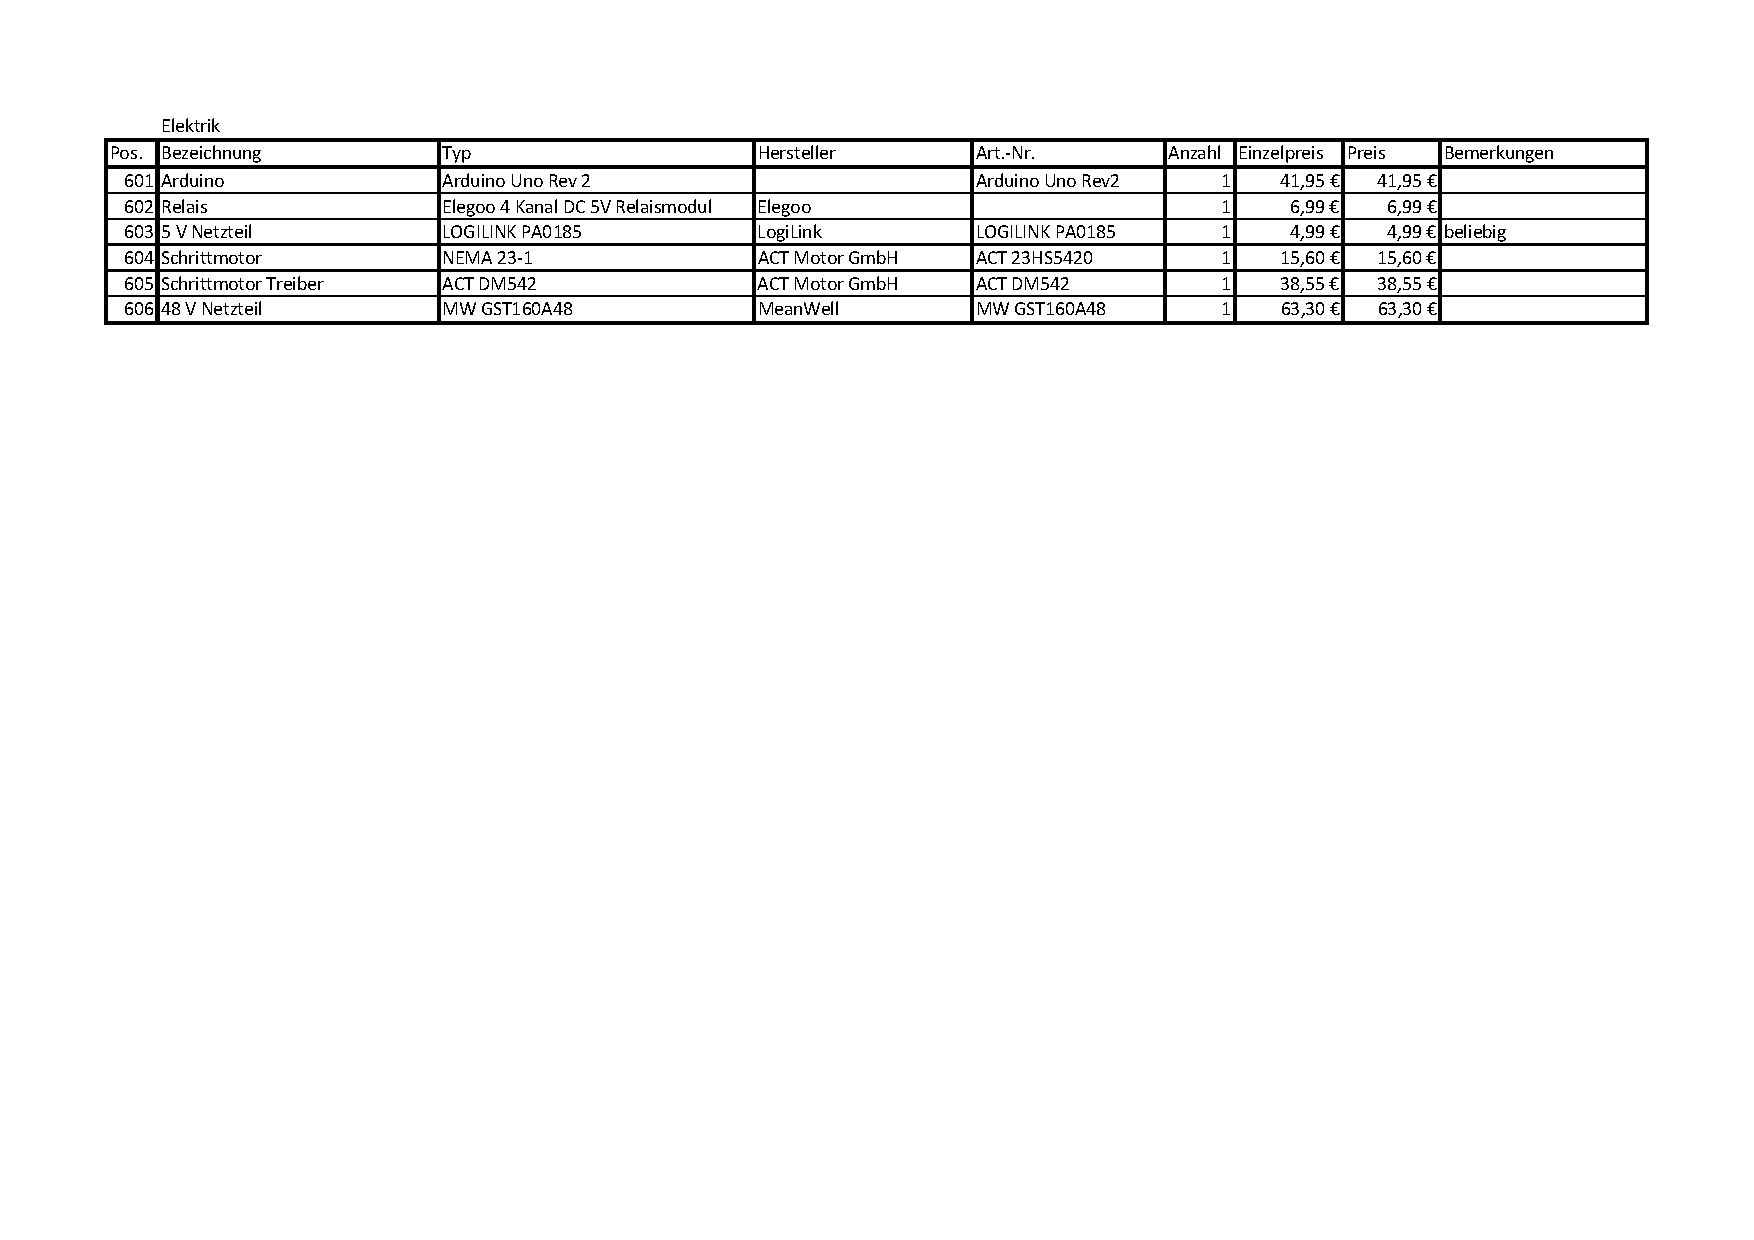
\includepdf[pages=-, angle=90, pagecommand={\thispagestyle{plain}}, addtolist={1, table, Stückliste Elektrik, tab:StuecklisteElektrik}]{Abb/Stuecklisten/StuecklisteElektrik.pdf}
%
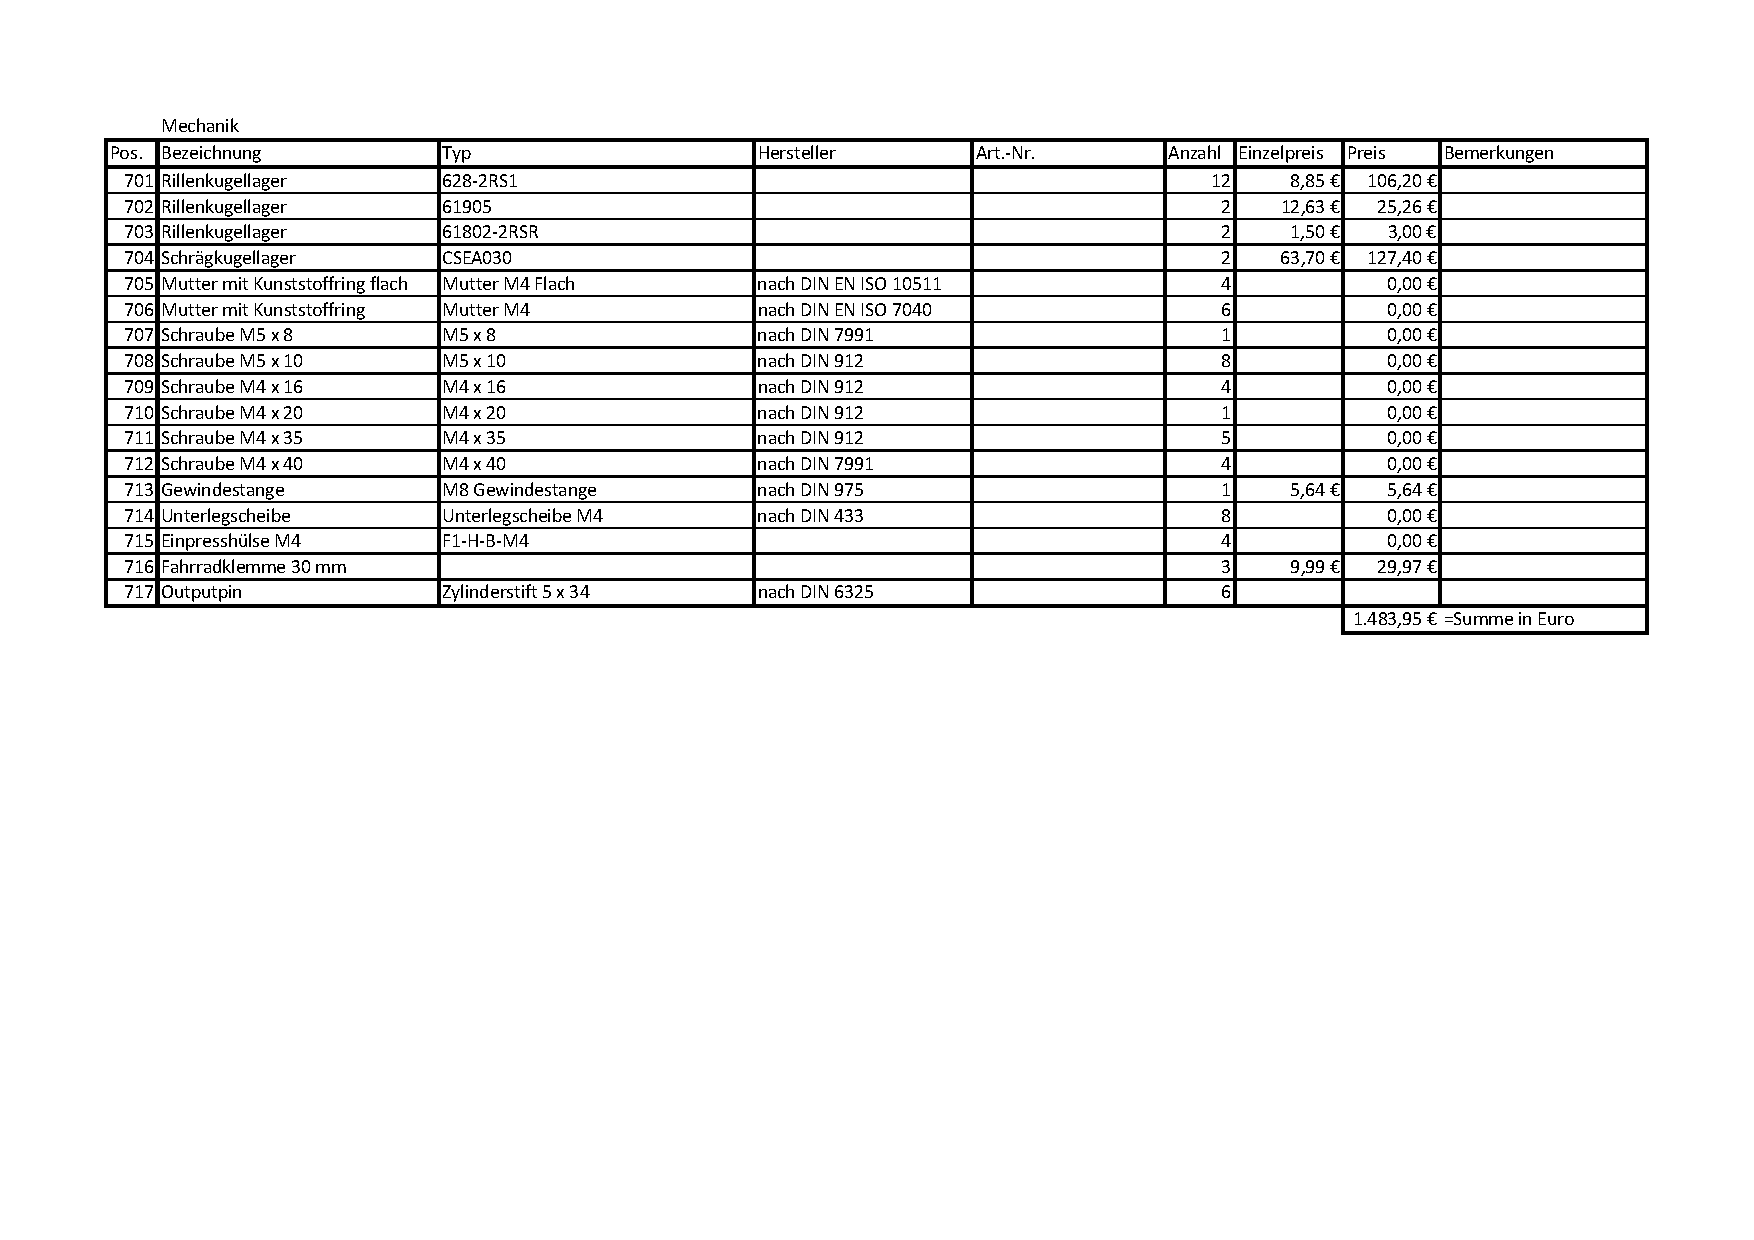
\includepdf[pages=-, angle=90, pagecommand={\thispagestyle{plain}}, addtolist={1, table, Stückliste Mechanik, tab:StuecklisteMech}]{Abb/Stuecklisten/StuecklisteMech.pdf}
\newpage
\setlength{\voffset}{-2.5 cm}
\setlength{\hoffset}{-2 cm}